% Document: A Simple Definition of Transfer Factors for Unramified Groups
% Author  : Thomas C. Hales, University of Chicago, hales@zaphod.uchicago.edu
% Typists : Fred Flowers and Thomas C. Hales
% First Draft: February 1991
% Corrected: July 7, 1992  (using errata of July 7, 1992)
% June 11, 2007 converted to LaTex.
% March 2015. LaTeX formatting updated.

% This file does not input any documents
% This is an AMS-TEX document.  
% There are no graphics but eight arrows have to be drawn into
%   a commutative diagram,  this is explained below in (9.2)
%   in a passage marked %%FIXX

% There is a separate document giving the bibliography

% Main changes in corrected version: 
%			Section 11 was rewritten to clarify the argument
% 			and the diagrams of section 14 were replaced by
%			descriptions of the diagrams.

% Format Instructions 


\documentclass{amsart}

%Packages
\usepackage{graphicx}
\usepackage{amsfonts}
\usepackage{enumitem}
\usepackage{amscd}
\usepackage{amssymb}
\usepackage{alltt}
\usepackage{txfonts}
%tikz graphics
%\usepackage{xcolor} % to remove color.
\usepackage{tikz} 
\usetikzlibrary{chains,shapes,arrows,shadings,trees,matrix,%
  positioning,intersections,decorations,%
  decorations.markings,decorations.pathmorphing,backgrounds,%
  fit,calc,fadings,decorations.pathreplacing}


%\theoremstyle{plain}
%\newtheorem{theorem}{Theorem}
%\newtheorem{lemma}[theorem]{Lemma}
%\newtheorem{problem}[theorem]{Problem}

%\theoremstyle{definition}
%\newtheorem{remark}[theorem]{Remark}
%\newtheorem{definition}[theorem]{Definition}

\newtheorem{thm}{}
\newenvironment{cthm}[1]
  {\renewcommand\thethm{\bf #1}\thm}
  {\endthm}


\newcommand{\ring}[1]{\mathbb{#1}}
\def\taglet#1{\text{\tt (#1)}}

% Now For the Definitions used in this paper
% The first few are redefinitions

\def\Re{{\Bbb R}}                          %Blackboard-bold R
\def\Ints{{\Bbb Z}}                          %Blackboard-bold Z
\def\Rats{{\Bbb Q}}                          %Blackboard-bold Q
\def\Nats{{\Bbb N}}                          %Blackboard-bold N

\def\Gal{\operatorname{\text{Gal}}}          %Operator Gal
\def\Com{{\Bbb C}}                         %Blackboard-bold C
\def\suchthat{\ {\vrule width1truept height.3truecm depth.1truecm}\ }
\def\Hom{\operatorname{Hom}}         %Operator Hom
\def\Def{\overset{\operatorname{def}}=}   %Symbol = by def
\def\varep{\varepsilon}
\def\Char{\operatorname{char}}               %Operator char
\def\what#1{\widehat#1}

\def\SL{\operatorname{SL}}
\def\bij{\buildrel{}\operatorname{bij}\over\leftrightarrow}
\def\adj{\operatorname{adj}}
\def\SP{\operatorname{Sp}}
\def\reschar{\operatorname{res.\,char.}}
\def\aff{\operatorname{aff}}
\def\Vol{\operatorname{vol}} 

\def\hgam{\gamma_H}
\def\ggam{\gamma_G}
\def\reg{\operatorname{reg}}

\def\GL{\operatorname{GL}}
\def\tild#1{\widetilde#1}
\def\sc{\operatorname{sc}}
\def\Waff{W_{\operatorname{aff}}}
\def\Waffsc{W_{\operatorname{aff,sc}}}
\def\map{\buildrel{}\widetilde{}\over\longrightarrow}
\def\Liet{\operatorname{Lie}(T)}               
\def\CurlyS{{\mathcal S}}             
\def\CurlyC{{\mathcal C}}            

% The following are used in citations

\def\ASSEM{1}
\def\BOREL{2}
\def\CARTER{3}
\def\CASSELMAN{4}
\def\CLOZEL{5}
\def\CLOZELSBC{6}
\def\DELIGNE{7}
\def\DERIZIOTIS{8}
\def\HALESU{9}
\def\HALESO{10}
\def\HALEST{11}
\def\HOWE{12}
\def\IWAHORI{13}
\def\IWASAWA{14}
\def\KAZHDAN{15}
\def\KOTTWITZS{16}
\def\KOTTWITZR{17}
\def\LABESSEF{18}
\def\LABESSEC{19}
\def\LANGLANDSO{21}
\def\LANGLANDSD{22}
\def\LANGLANDSCAN{20}
\def\MACDONALD{23}
\def\SHELSTAD{24}
\def\WALDSPURGER{25}
\def\WALDSPURGERL{26}


\begin{document}


%\centerline{\bf A SIMPLE DEFINITION OF TRANSFER FACTORS}
%\centerline{\bf FOR UNRAMIFIED GROUPS}\vskip6pc
%\baselineskip=10pt
%\centerline{\bf Thomas C. Hales}\vskip1pc
%\centerline{\bf University of Chicago}\vskip1pc
%\centerline{\bf February 5, 1991}\vskip1pc
%\centerline{\bf Corrected July 7, 1992}\vskip6pc


\begin{abstract}
This paper gives simple characterization
of transfer factors for unramified groups which is shown to be equivalent
to the definition of Langlands and Shelstad  under mild restrictions on the
residual field characteristic.
\end{abstract}

%\vfil\eject
\title{A Simple definition of transfer factors for unramified groups}
\author{Thomas C. Hales}
\address{University of Chicago}
\date{February 5, 1991; corrected July 7, 1992}
\thanks{CONTEMPORARY MATHEMATICS 145 (1993): 109-134.}
\maketitle

%\baselineskip=2\baselineskip

\noindent PART I PRELIMINARIES\smallskip
\begin{enumerate}[label=]
\item{1.}  Introduction
\item{2.}  Compact Elements
\item{3.}  Topological Jordan Decomposition
\item{4.}  Centralizers of Semisimple Elements
\item{5.}  Abelian Class Field Theory
\item{6.}  Embeddings of $L$-Groups\medskip
\end{enumerate}

\noindent PART II  TRANSFER FACTORS\smallskip

\begin{enumerate}[label=]
\item{7.}  Canonical Normalization of Transfer Factors
\item{8.}  Coherence of Canonical Normalization
\item{9.}  Descent for Levi Factors
\item{10.}  Homogeneity and General Descent
\item{11.}  Central Characters\medskip
\end{enumerate}


\noindent PART III  ORBITAL INTEGRALS\smallskip

\begin{enumerate}[label=]
\item{12.}  Harish-Chandra Descent
\item{13.}  Descent for Absolutely Semisimple Elements
\item{14.}  Regular Unipotent Orbital Integrals
\end{enumerate}
\vfil\eject

\centerline{\bf PART I.\ \  PRELIMINARIES}\vskip3pc
\section{Introduction} %1

Transfer factors have been defined for arbitrary
reductive groups in \cite{\LANGLANDSO}. When the group $G$ and the endoscopic
group $H$
are unramified, it is possible to give a simple
characterization of the transfer factors when we place
mild restriction on the residual characteristic.

The following rules, which are described precisely in the body of this
paper, give a complete characterization of the transfer factor for
unramified groups on the subgroup $G_{der}(F)Z_G^0(F)$ of finite
index in $G(F)$.
The endoscopic group determines a character
$\kappa:H^1(\Gal(\overline F/F),T(\overline F))\to \Com^\times$.

{1.} The transfer factor at a noncompact 
element $g$ coincides with the product of the transfer factor for a proper
Levi subgroup of $G$ containing $g$ with a relative discriminant factor (9.2).

{2.} The transfer factor on compact elements is an explicit
unramified character on the center of
$G$ times the transfer factor on strongly compact elements (11.1), (11.2), (11.3).

{3.}  The transfer factor on strongly compact 
elements $g$ coincides with the transfer factor of
the centralizer of the absolutely semisimple part of $g$ (10.18).

{4.} The transfer factor on topologically unipotent elements
is obtained by homogeneously extending the transfer
factor defined near regular unipotent elements (10.17).

{5.}  The transfer factor near a regular unipotent element
$u^g$ is given by $\kappa_0(\sigma(g)g^{-1})$ times a relative discriminant
factor for an
explicit character $\kappa_0$ on $H^1(\Gal(\overline F/F),Z_G)$
provided $u$ is an element which is regular modulo $p$ and
$\sigma(g)g^{-1}\in Z_G$, $\sigma\in\Gal(\overline F/F)$ (Section 14).
$\kappa_0$ is the restriction of $\kappa$ to the center of $G$.
This character is trivial, for instance, if $G$ is an adjoint group.

{6.}  The transfer factor at $\gamma^g$, with $\gamma$ strongly regular semisimple
and $g\in (T\backslash G)(F)$, is
given by $\kappa(\sigma(g)g^{-1})$ times the transfer factor at $\gamma$.

Rules 5 and 6 may be replaced by the cohomological description of the 
Shalika germs for the regular unipotent conjugacy class
obtained by Shelstad \cite{\SHELSTAD}.

 Rules 5,6  give the transfer factor near the identity, rule 4 extends 
it to all topologically unipotent elements, rule 3 extends it to 
strongly compact elements, and rule 2 extends it to compact elements.
Finally, rule 1 gives the transfer factor in terms of its values on
compact elements.

The rules 1--6 are given in a form that I hope will be 
amenable to the study of the fundamental lemma,
for parallel to each of these rules is an
established fact about
 the orbital integrals
of the unit element of the Hecke algebra:
{1.}  The orbital integral of a non-elliptic element
$g$ coincides with the orbital integral on a proper Levi
subgroup of $G$ containing $g$.
{2.}  The orbital integral of suitable compact elements is an 
explicit unramified character of the center of $G$
times the orbital integral on a strongly compact element.

{3.} The orbital integral of a strongly compact
element $g$ coincides with the orbital integral of the centralizer
of the absolutely semisimple part of $g$.

{4.}  The Shalika germs of orbital integrals are homogeneous
functions sufficiently close to the identity element.

{5.}  the $\kappa$-orbital integral of a regular unipotent class 
coincides with the stable orbital integral on the regular
unipotent class of the endoscopic group.\par

Statement 1 is known as Harish-Chandra descent, statement 2 is
trivial. The character appearing in statement 2
is the same as the character in rule 2 above.
 Statement 3 is a lemma of Kazhdan/Kottwitz; statement 4 is due to
Harish-Chandra, and statement 5 is formulated precisely and
proved in this paper (14.2).  To prove the fundamental lemma it would suffice
to prove a stronger version of statements 4 and 5.  

The main ingredient missing
that prevents us from proving the fundamental lemma much more generally is the
homogeneity of Shalika germs for all topologically unipotent elements for
functions in the Hecke algebra.   Assuming homogeneity, to establish the
fundamental lemma for the identity of the Hecke algebra it would be sufficient
to prove the fundamental lemma either for elements sufficiently close to the
identity or for elements at the other extreme: nearly absolutely
semisimple.  Thus the fundamental lemma would follow from homogeneity together
with either a knowledge of the Shalika germs or an improved version of a lemma
of Kazhdan \cite{{\KAZHDAN}}.  These are the two approaches taken 
in \cite{{\HALESU,\WALDSPURGER}}
for the group $SL(n)$ (where homogeneity of germs is known).  In both
approaches the simple formulation of the transfer factor provided here
plays an important role.  For example, the results of this paper imply that
for $SL(n)$ the transfer factor on strongly compact elements is simply the
quotient of the
discriminant factors for $SL(n)$ and $H$,  when the endoscopic group $H$ 
splits over an unramified extension of odd degree.

An approach based on unipotent orbital integrals, the trace formula, or local character
identities 
\cite{{\ASSEM,\CLOZELSBC,\LABESSEF,\WALDSPURGER}}, might make
it possible to deduce the fundamental lemma from the matching of the
unit element of the Hecke algebra.

The transfer factors were designed
with the fundamental lemma and a number of other 
constraints in mind.  It is evidence of the power and foresight of
the definition of Langlands and Shelstad that a factor designed for
many purposes should serve so well its purpose in this context.

I would like to thank R. Kottwitz, R. Langlands and
J. Rogawski for helpful comments.\medskip

\noindent {\bf Assumptions and Notation.}
Let $F$ be a $p$-adic field of characteristic zero.
We assume $\reschar F\ne 2$.  Let $O_F$ denote the
ring of integers of $F$.  Let $G$ be a connected reductive
group over $O_F$.  We assume that $G(O_F)$ is a 
hyperspecial maximal compact subgroup of $G(F)$ (modulo the
center) and that $G/F$ is quasi-split
and splits over some unramified extension $E$ of $F$.  
Let $\pi$ be a prime element of $O_F$.  Let $q$ be the 
cardinality of the residue field of $F$ and let $p$
denote the rational prime dividing $q$.  We let
$\tilde{}:G(O_F)\to G(\Bbb F_q)$, $g\mapsto\tilde g$, denote 
reduction modulo the maximal ideal $(\pi)$.  Let
${}^LG=\widehat G\rtimes\Gal(E/F)$ be the dual group of $G$.
Let $F^u$ denote a maximal unramified extension of $F$, and let $\overline F$ be
an algebraic closure of $F$.  Let $\Bbb T_G$ be a
maximally split Cartan subgroup of $G$, and let $\Bbb B$ be a Borel subgroup
over $F$ containing $\Bbb T_G$.  Define $\Bbb T_H$ similarly for an endoscopic
group $H$ of $G$.  If $H$ splits over an unramified extension then $\Bbb T_H$
is also unramified.  We often identify $\Bbb T_H$ with an isomorphic
Cartan subgroup of $G$.

\section{Compact Elements} %2.

We say that $g\in G(F)$ is {\it strongly compact\/} if
the following equivalent conditions hold:

{1.} $g$ lies in a compact subgroup of $G(F)$.

{2.}  The eigenvalues of $\rho(g)$ are units in
$\overline F$ for some faithful finite-dimensional
rational representation $\rho:G\to\GL(V)$ defined over $\overline F$.\par



We say that $g\in G(F)$ is {\it compact\/} if its image in
$G_{\adj}(F)$ is a strongly compact element of 
$G_{\adj}(F)$.  This definition of compact
coincides with the usage of \cite{{\CASSELMAN,\CLOZEL,\DELIGNE}}.
Every strongly compact element is compact.

If an element is not compact then it is not elliptic and we may select a Levi factor
$M$ of $G$ such that it is elliptic in $M$.

\section{Topological Jordan Decomposition} %3.

This section reviews some properties of the topological Jordan
decomposition \cite{{\KAZHDAN,\WALDSPURGERL}}.  If $K$ is a 
profinite group with a normal pro-$p$-group $L$ of finite index
then the prime-to-$p$ part of the order of $K/L$ is an integer 
independent of the choice of $L$ which we denote by $c_K$.  If 
$G$ is a reductive $p$-adic group then it has only finitely
many maximal compact subgroups up to conjugacy 
$K_1,\ldots,K_f$ and we let $c=c_G$ be
the least common multiple of the $c_{K_i}$.  

We define an absolutely semisimple element in $G$
to be a semisimple element $\gamma$ such that
$\gamma^c=1$.  Such elements are strongly compact.
We define a topologically unipotent element $\gamma$ of $G(F)$ to be
an element such that $\lim_{m\to\infty}\gamma^{q^m}=1$.
Such elements are also strongly compact.  For each strongly compact
element $\gamma$ we define a decomposition, called the topological
Jordan decomposition,  $\gamma=\gamma_s\gamma_u
=\gamma_u\gamma_s$ into absolutely semisimple $\gamma_s$
and topologically unipotent element $\gamma_u$ as follows. 
Let $\ell$ be a positive integer such that 
$q^\ell\equiv1\mod c$.  Set 
$\gamma_s=\lim_{m\to\infty}\gamma^{q^{\ell m}}$
and $\gamma_u=\gamma\gamma_s^{-1}$.  It is readily verified
that this limit exists \cite{\IWASAWA}.  One can
verify without difficulty that the following properties hold:

{1.}   $\gamma_s\in G(F)$ is absolutely semisimple.

{2.} $\gamma_u$ is topologically unipotent.

{3.} If $\gamma=\gamma_s^\prime\gamma_u^\prime
=\gamma_s\gamma_u$
are two decompositions into commuting absolutely semisimple and
topologically unipotent elements then $\gamma_s
=\gamma_s^\prime$ and $\gamma_u=\gamma_u^\prime$.

{4.} If $\rho:G\to G^\prime$ is a morphism of reductive groups
defined over a finite extension of $F$ then $\rho(\gamma)_s=\rho(\gamma_s)$,
$\rho(\gamma)_u =\rho(\gamma_u)$. In particular :

item{a.} 
If $E$ is a finite  extension of $F$
then the topological Jordan decomposition is the same
for strongly compact elements of $G(F)$ whether viewed as elements of
$G(F)$ or $G({E})$.

item{b.}
$(\gamma^g)_u = (\gamma_u)^g$, $(\gamma^g)_s = (\gamma_s)^g$.

{5.} If $G=\GL(1)$
then $\gamma\mapsto\gamma_s$,
$\gamma\in O_F^\times$ is the Teichm\"uller 
character of $O_F^\times$ \cite{\IWASAWA}.

{6.}  Let $H$ be an endoscopic group satisfying
the same conditions as $G$ (that is, defined over $O_F$, unramified,
etc). Suppose that $\gamma\in G(O_F)$ is an image of
some strongly $G$-regular semisimple element 
$\gamma_H\in H(O_F)$ then
$\gamma_s$ is a $C_G(\gamma)$-image of 
$\gamma_{H,s}$ (for terminology see \cite{\LANGLANDSO}).

{7.} If $\gamma\in G(O_F)$, then $\widetilde \gamma=\widetilde\gamma_s\widetilde\gamma_u$
is the Jordan decomposition of $\widetilde\gamma\in G({\Bbb F_q})$.
\par
\smallskip

If $F/\Rats_p$ is a finite extension then define $e_F$ to be the ramification
degree of $F$ over $\Rats_p$.  If $T$ is a Cartan subgroup, define $e_T$ to be
the minimum of $e_E$ over all fields $E$ splitting $T$.  Finally if $G$ is a
reductive group, define $e_G$ to be the maximum of $e_T$ as $T$ ranges over all
Cartan subgroups defined over the ground field.  Also write $U(F)$ for the topologically
unipotent elements of $F^\times$.

\begin{cthm}{Lemma 3.1}  Suppose $p> e_F+1$ and $x$ is topologically
unipotent in $F^\times$.
If $Q=p^\ell$, $\ell>0$, then $(x^Q-1)/Q(x-1)$ is topologically unipotent.
\end{cthm}

\begin{proof}
By the binomial theorem, $(1+y)^Q-1 = yQ(1+\sum_{i=2}^Q 
\frac1Q{Q\choose i}y^{i-1})$, where $x=1+y$.

For $1\le k< Q$, $(Q-k)/(-k)$ is topologically unipotent.
So $\frac1Q{Q\choose i}=u_i(-1)^{i-1}/i$ with $u_i$ topologically
unipotent.  The lemma will follow if 
$|{y^{i-1}}/i|<1$ for $i\ge2$.
The worst case is
$y=\pi$, $(i)=(p^r)=(\pi^{er})$. Then  $y^{i-1}/i$
behaves as $\pi^{p^r-1-er}$.  The worst case is $r=1$. So we need
$|\pi^{p-1-e}|<1$ or $p>e_F+1$.
\end{proof}

\begin{cthm}{Remark 3.2}  The condition for the exponential power series
to converge on $U(F)-1$ is $p>e_F+1$. Also the
logarithmic power series  converges on $U(F)$ to an element of $U(F)-1$ if $p>e_F$.
\end{cthm}

The topological Jordan decomposition leads to the
following decomposition of a field.
If $E$ is any finite extension of $F$, then $E^\times \map \langle\pi_E\rangle
\times A_E\times U(E)$, with $\pi_E$ a uniformizer,
$A_E$ absolutely semisimple, and
$U(E)$ topologically unipotent.
If the ramification degree of $E$ over $F$ is $e$ then
we take $\pi=\pi_E^e$ as a uniformizer of $F$.
Then 
\[
\begin{CD} F^\times@>\sim>> \langle\pi\rangle\times A\times U(F)\end{CD},
\]
where 
$A\subseteq A_E$ absolutely semisimple,
$\langle\pi\rangle\subseteq\langle\pi_E\rangle$, and 
$U(F)\subseteq U(E)$ is topologically unipotent.

\begin{cthm}{Definition}  We say a character $\theta$ on $F^\times$
is tamely ramified if $\theta(U(F)) = 1$.
\end{cthm}

\begin{cthm}{Lemma 3.3}  Let $\theta$ be a tamely ramified character
of $F^\times$ and let $E$ be a finite extension of $F$.  Then
there is a tamely ramified character on $E^\times$ extending $\theta$.
\end{cthm}

\begin{proof}  
Take the extension to be trivial on $U(E)$ and arbitrary extensions 
on $A_E$, $\langle\pi_E\rangle$.
\end{proof}

\section{Centralizers of Semisimple Elements} %4.

In this section, let $G$ be a complex semisimple group.
Let $T$ be a maximal torus of $G$ with Lie
algebra $\Liet$.  We let $G_{\operatorname{adj}}$ and 
$G_{\sc}$ be the corresponding adjoint and simply-connected groups.
Let $\tild\Delta =\Delta\cup\{-r_0\}$ be the extended system of
simple roots for $T$.  Let $\exp:\Liet\to T$ be the exponential map,
and let $X_*$ be the kernel of this map.  $X_*$ acts on $\Liet$
by translation $\mu.Y=\mu+Y$. We also set 
$\exp_{\sc}:\Liet\to T_{\sc}\subseteq G_{\sc}$,
$X_{*,\sc}=\ker(\exp_{\sc}:\Liet\to T_{\sc})$.  Let $W$ be the 
Weyl group for $T$.  Let $\Waff= X_*\rtimes W$ be the affine Weyl group,
and $\Waffsc = X_{*,\sc}\rtimes W$.
Two elements $Z,Y\in \Liet$ have conjugate images
$\exp(Z)^g = \exp(Y)$, $g\in G$, if and only if
$w.Z=Y$ for some $w\in \Waff$.  Let $\CurlyC$ be a fundamental chamber
for the action of $\Waffsc$ on $\Liet$.  For 
$Y\in \CurlyC$ let $\CurlyC_Y$ be the smallest facet of $\CurlyC$
containing $Y$.  Let $\Omega=\{w\in\Waff
\suchthat w\CurlyC=\CurlyC\}$, then by \cite{\IWAHORI}
$$
\Waffsc\rtimes\Omega
\map
\Waff.
$$

For the next few lemmas set $s=\exp(Y)$, $Y\in \CurlyC$.
\begin{cthm}{Lemma 4.1}    The inclusion $C_{N_G(T)}(s)\subseteq
C_G(s)$ induces an isomorphism between
$
C_{N_G(T)}(s)/(C_{N_G(T)}(s)\cap C_G(s)^0)$ and $C_G(s)/C_G(s)^0$.
\end{cthm}

\begin{proof} \cite{\CARTER}
\end{proof}

\begin{cthm}{Lemma 4.2} 
$
C_{N_G(T)}(s)\cap C_G(s)^0/T\map C_{\Waffsc}(Y)
$.
\end{cthm}

\begin{proof}  If $n\in C_G(s)^0\cap C_{N_G(T)}(s)$ then
lift $n$ to $\widehat n\in G_{\sc}$, and $s$ to $\widehat s$.  Then 
$\widehat n\widehat s\widehat n^{-1}=\widehat s$.  So
$\widehat n\in C_{G_{sc}}(\widehat s) = C_{G_{sc}}(\widehat s)^0$ \cite{\CARTER}.
Thus
$$
C_G(s)^0\cap C_{N_G(T)}(s) =
\operatorname{image}\left(
C_{N_{G_{\sc}}(T_{\sc})}
(\widehat s)\to G\right).
$$
If $n\in C_{N_{G_{\sc}(T_{\sc})}}(\widehat s)$,
then its image $w$ in $W$ acts on $Y$
by $wY =\mu Y$, $\mu\in X_{*,\sc}$.  So replacing
$w$ by $w\mu^{-1}$ we obtain a surjection
$C_{N_{G_{\sc}}(T_{\sc})}(\widehat s)\to C_{\Waffsc}(Y)$.
The isomorphism follows easily.
\end{proof}
Similarly,
\begin{cthm}{Lemma 4.3}$C_{N_G(T)}(s)/T\map C_{\Waff}(Y)$.
\end{cthm}

Thus,
\begin{cthm}{Corollary 4.4} $C_G(s)/C_G(s)^0\map
C_{\Waff}(Y)/C_{\Waffsc}(Y)$.
\end{cthm}

\begin{proof}  Lemmas 4.2 and 4.3.
\end{proof}

In the disconnected case, set 
$G^\prime = G\rtimes I$ and 
$G_{\sc}^\prime=G_{\sc}\rtimes I$,
where $I$ is a finite group of outer automorphisms
of $G$, $G_{\sc}$ fixing $T$, $T_{\sc}$.  Set
$W^\prime = W\rtimes I$, 
$W_{\operatorname{aff}}^\prime = X_*\rtimes W^\prime$,
$\Omega^\prime = \{w\in W_{\operatorname{aff}}^\prime
\suchthat w\CurlyC = \CurlyC\}$.  Set $\Omega^\prime_Y = \{w\cdot Y=Y\}$.
Assume that $I$ acts in such a way to stabilize $\CurlyC$, so that $I\subseteq\Omega'$. We obtain as in the 
connected case

\begin{cthm}{Lemma 4.5}
$
C_{G^\prime}(s)/C_{G^\prime}(s)^0
\map C_{\Waff^\prime}(Y)/C_{\Waffsc}(Y)
\map\Omega_Y^\prime\subseteq\Omega^\prime.
$
\end{cthm}

\begin{cthm}{Lemma 4.6} The following exact sequence splits.
$$
1\to C_{\Waffsc}(Y)\to
C_{\Waff^\prime}(Y)
\to \Omega_Y^\prime\to 1.
$$
\end{cthm}

\begin{proof}  $C_{\Waffsc}(Y)$ is
the Weyl group of reflections stabilizing
$\CurlyC_Y$ the smallest facet of $\CurlyC$ containing $Y$.
It acts transitively on the set of chambers 
containing $\CurlyC_Y$.  Thus if $w\in C_{\Waffsc}(Y)$
then $w\cdot Y=Y$, and $w\cdot \CurlyC_Y = \CurlyC_Y$.
Select $w^\prime\in C_{\Waffsc}(Y)$ such that
$w^\prime w\cdot \CurlyC = \CurlyC$; then
$w^\prime w\in\Omega^\prime$ gives the 
splitting.  
\end{proof}



For each $\omega\in \Omega^\prime$, let
$n_\omega\in N_G(T)\rtimes I$ be an element such that
$$
n_\omega\mod T \qquad=\quad\omega\mod X_*\in W\rtimes I.
$$
Combining all of the previous results we obtain the following theorem.  It
tells us that the components of $C_{G^\prime}(s)$ are represented by elements
$n_\omega$ independent of $s$.

\begin{cthm}{Theorem 4.7} Let $s=\exp(Y)$, $Y\in \CurlyC$, be 
semisimple.  
Then
$$
C_{G^\prime}(s) = C_G(s)^0\{n_\omega\}_{\omega\in\Omega_Y^\prime}.
$$
\end{cthm}

\section{Abelian Class Field Theory} %5

In this section, we recall Labesse's version \cite{\LABESSEC} of the isomorphism
between
$$
\Hom_c(T(F),\Com^\times)\quad\text{and}\quad
H_c^1(W_{E/F},\widehat T(\Com))
\qquad (c =\text{ continuous})
$$
where $E$ is a Galois extension which splits $T$.  Set
$\Gamma=\Gal(E/F)$, $X_* =$ cocharacters of $T(\overline F)$
viewed as a $\Gamma$-module, $W_{E/F}$ the Weil group, $\widehat T$ the
complex dual of $T$. We start with the 
surjective corestriction map:
$$
\begin{CD}
H_c^1(E^\times,\widehat T)@>{\text{Cor}}>> H_c^1(W_{E/F},
\widehat T)\taglet{1}
\end{CD}
$$
corresponding to the short exact sequence
$
1\longrightarrow E^\times\longrightarrow W_{E/F}\longrightarrow
\Gamma\longrightarrow 1.
$
If $\{w_\sigma\}_{\sigma\in\Gamma}$ are 
representatives in $W_{E/F}$ of the elements
of $\Gamma$, then
$\text{Cor}\varphi(w)\Def\sum_{\sigma\in\Gamma}
w_\tau\varphi(w_\tau^{-1}ww_\sigma)$
where $\tau=\tau(\sigma)\in \Gamma$ is defined by
$w_\tau^{-1}ww_\sigma\in E^\times$.  We have
$$
\begin{array}{lll}
H_c^1(E^\times,\widehat T) &=
\Hom_c(E^\times,\widehat T)\taglet2\\
&=\Hom_c(E^\times,\Hom(X_*,\Com^\times)) \taglet3\\
&=\Hom_c(E^\times\otimes X_*,\Com^\times) \taglet4\\
&=\Hom_c(T(E),\Com^\times) \taglet5\\
\Hom_c(T(E),\Com^\times) &\twoheadrightarrow
\Hom_c(T(F),\Com^\times). \taglet6
\end{array}
$$

If we now replace each of the groups $A$ in lines 2--5
by $H_0(\Gamma,A)\Def A/I_\Gamma A
=A/\{\sigma a-a\suchthat
a\in A, \sigma\in \Gamma\}$
then the maps in lines 1 and 5 descend to the
quotient in homology and become isomorphisms.
This gives the desired isomorphism between
$H_c^1(W_{E/F},\widehat T)$ and
$\Hom_c(T(F),\Com^\times)$.  For proofs see \cite{\LABESSEC}.
By the explicit form of the isomorphism in lines
2--6 we see 

\begin{cthm}{Lemma 5.1}  Suppose that
$\varphi\in Z_c^1(E^\times,\widehat T)
=H_c^1(E^\times,\widehat T)
=\Hom_c(E^\times,\widehat T)$
is tamely ramified.  Then the corresponding homomorphism in
$\Hom_c(T(F),\Com^\times)$
(obtained by the maps in lines 2--6) is
also tamely ramified.
\end{cthm}

\section{Embeddings of $L$-Groups} %6

Let $(H,\mathcal{ H},s,\xi)$ be endoscopic data for $G$
(see \cite{\LANGLANDSO}).  
We say that $(H,\mathcal{ H},s,\xi)$ is {\it unramified }
endoscopic data for $G$ if 
{1.}  $G$ is defined over $O_F,G(O_F)$ is hyperspecial,
and $G$ splits over an unramified extension of $F$.

{2.}  $H$ is defined over $O_F,H(O_F)$ is hyperspecial,
and $H$ splits over an unramified extension of $F$.

{3.}  $\mathcal{ H}={}^LH$ is the $L$-group of $H$.

{4.}  $(H,\mathcal{ H},s,\xi)$ is endoscopic data for $G$.

{5.}  The embedding $\xi$ descends to some finite unramified
extension $E/F$.  
In other words we have a commutative diagram
$$
\begin{CD}
{}^LH @>\xi>> {}^LG\\
@V\varphi_H VV    @V\varphi_GVV\\
\widehat H\rtimes\Gal(E/F) @>{\xi_0}>> 
\widehat G\rtimes \Gal(E/F)
\end{CD}
$$
The maps $\varphi_H,\varphi_G$ are induced by the canonical projection
$\varphi:W_F\to \Gal(E/F)$.

For the next lemma we make a series of assumptions.
Suppose $H$ is an unramified reductive group defined over $F$.
Suppose that 
$\widehat H=C_{\widehat G}(s)$ for some semisimple element
$s\in\widehat G$.  Suppose also that for every $\sigma\in \Gal(E/F)$ there
is an element $\omega(\sigma)\rtimes\theta$ in ${}^LG$ such that the action
of $\sigma$ as an outer automorphism of $\widehat H$ coincides with the
outer automorphism defined by conjugation by $\omega(\sigma)\rtimes\theta$.

\begin{cthm}{Lemma 6.1}  Under the assumptions above, there exists an embedding
$\xi:{}^LH\to{}^LG$ that makes $(H,{}^LH,s,\xi)$ into
unramified endoscopic data.
\end{cthm}

\begin{cthm}{Remark}  This lemma is not true without the assumption that $H$ is
unramified.  In fact the purpose of \cite{\LANGLANDSCAN} is to circumvent
this lemma in the ramified case.
\end{cthm}

\begin{proof}  The group ${}^LH$ is
defined by some $\widehat H\rtimes\Gal(E/F)$,
$E/F$ unramified.  Let $\sigma$ be a generator of 
$\Gal(E/F)$.  Let $\omega(\sigma)$ be in the Weyl group such that
$\sigma$ acts on $\widehat H$ by $\omega(\sigma)\rtimes\theta$
with $\theta$ outer in $\widehat G$. We may assume
$\omega(\sigma)$, $\sigma$ and $\theta$ act as 
automorphisms of extended Dynkin diagrams and stabilize $\widehat B_H$,
$\widehat T_H$ (Borel and Cartan for $\widehat H$).  Then
$w=n(\omega(\sigma))\rtimes\theta$ also stabilizes $\widehat B_H$,
$\widehat T_H$.  Here $n(\cdot)$ is a representative in the normalizer
defined in \cite{\LANGLANDSO}.  By construction $w$
is of finite order $k$.  In fact, 
$w^{[E:F]}$ has order 2 \cite{\LANGLANDSO}.
Let $O_1,\cdots,O_r$ be the orbits
of the positive simple roots of $H$ under $\langle w\rangle$.
For each orbit $O_i$ pick $t_i\in \widehat T_H$ of finite order such that
$\alpha(t_i)=1$ for $\alpha\not\in O_i$ and for which there exist root
vectors $\{X_\alpha\}$, $\alpha\in O_i$ stable under $t_iw$.  Then
$w' = (\prod t_i)w$ is of finite order $k'$ and stabilizes the set of root vectors
for simple roots of $\widehat H$.  Let $E'$ be the unramified extension of $F$
of degree $k^\prime$, and $\sigma'$ a generator of $\Gal(E'/F)$ over $\sigma\in\Gal(E/F)$. 
Then define
$
\xi_0:\widehat H\rtimes\Gal(E'/F)
\to \widehat G\rtimes\Gal(E'/F)
$
by $\xi_0(\sigma') =w^\prime$.  This gives $\xi$.
\end{proof}
\vfil\eject 

\centerline{\bf PART II.  TRANSFER FACTORS}\bigskip

\section{Canonical Normalization of Transfer Factors} %7

By our assumptions on $G$ we may assume $G=G^*$ (quasi-split
inner form) and that the inner twist $\psi:G\to G^*$ to the
quasi-split form is the identity.  To each $G$ and set
of unramified endoscopic data $(H,{}^LH,s,\xi)$ we define
a canonical transfer factor $\Delta_0(\gamma_H,\gamma_G)$.
Recall that the transfer factor $\Delta_0$ of \cite{\LANGLANDSO}
depends on a choice of splitting.  We will use the
subgroup $G(O_F)$ to determine a splitting.

\begin{cthm}{Definition 7.1}  We say that a splitting 
$(B,T,\{X_\alpha\})$ is admissible if the following conditions hold:
{1.}  $B$ and $T$ are Cartan subgroups over $F$.
{2.}  If $u_\alpha$ is the homomorphism
$u_\alpha:\Bbb G_a\to G$ determined by $X_\alpha$ then
$u_\alpha$ is defined over $O_{F^u}$ and $\tilde u_\alpha(1)$
is not the identity element in $G(\overline{\Bbb F}_q)$.
\end{cthm}

We define $\Delta_0(\gamma_H,\gamma_G)$ to be the transfer
factor $\Delta_0(\gamma_H,\gamma_G)$ of \cite{\LANGLANDSO} defined
relative to an admissible splitting of $G$.

\begin{cthm}{Lemma 7.2}  $\Delta_0(\gamma_H,\gamma_G)$ is independent
of the admissible splitting of $G$.
\end{cthm}

\begin{proof}  $\Delta_I(\gamma_H,\gamma_G)$ is the only term
of the transfer factor depending on a splitting and
$\Delta_I(\gamma_H,\gamma_G)/\Delta_I(\overline\gamma_H,
\overline \gamma_G)$ is independent of the splitting of $G$.
Thus it is enough to prove the independence of the admissible
splitting for a pair $\gamma_H,\gamma_G$ of our choice.  We
take $\gamma_H$ to lie in the unramified maximal split torus $\Bbb T_H$ of $H$.
Identify $\Bbb T_H$ with an isomorphic Cartan subgroup of $G$.  With
an appropriate choice we may identify $\Bbb T_H(O_F) = H(O_F)\cap \Bbb T_H(F)$
with $G(O_F)\cap \Bbb T_H(F)$. 
With an unramified Cartan
subgroup we are allowed to take all our $a$-data to be units in an
unramified extension of $F$.  Since $u_\alpha$ is defined over
$O_{F^u}$ and $\tilde u_\alpha(1)\ne1$, the coroots $\alpha^v:\Bbb G_m\to G$
and negative roots $u_{-\alpha}:\Bbb G_a\to G$ are also defined
over $O_{F^u}$.  Hence \cite{\LANGLANDSO}	%p231,228
\begin{gather*}
x(\sigma_T)\Def\prod_{1,\sigma}^p
a_\alpha^{\alpha^v}\in G(O_{F^u})\\
n(\alpha)\Def\exp(X_\alpha)\exp(-X_{-\alpha})
\exp(X_\alpha)\in G(O_{F^u}).
\end{gather*}
Similarly $n(\omega)$ and $m(\sigma_T) = x(\sigma_T)n(\omega_T(\sigma))$ belong
to $G(O_{F^u})$.


Since the pair $(B,\Bbb T_H)$ is isomorphic to $(\Bbb B,\Bbb T_G)$ over
an unramified extension, and since our integral structures have been chosen
compatibly, 
we may select $h\in G(O_{F^u})$ such that 
$(B,\Bbb T_H)^h=(\Bbb B,\Bbb T_G)$.
 %page 231 of LS
Then the cocycle
$\sigma\mapsto hm(\sigma_T)\sigma(h^{-1})$
in $\Bbb T_H(\overline F)$ actually lands in 
$H^1(F^u,\Bbb T_H(O_{F^u}))=\{1\}$.  This cocycle
defines the element $\lambda(\Bbb T_H)=\lambda_{\{a_\alpha\}}(\Bbb T_H)$
so that 
$\lambda(\Bbb T_H) = 1$.  Hence
$\Delta_I(\gamma_H,\gamma_G)
\Def\langle\lambda(\Bbb T_{H,sc}),s_T\rangle=1$.  In particular,
it is independent of our choice of admissible splitting.
\end{proof}

\section{Coherence of Canonical Normalization} %8

Fix $\gamma_H\in H(O_F)$. We will assume that this element is
strongly compact and strongly $G$-regular. Set $\varep_H=\gamma_{H,s}$
and $\varep_G=\varep=\gamma_{G,s}$.  Let $\Delta_{\varep,0}$
be the canonical transfer factor associated to $(G_\varep,H_{\varep})$
as in \cite{\LANGLANDSD}.  In \cite{\LANGLANDSD} it is shown that
$\Delta_0(\gamma_H,\gamma_G) = c_\varep\Delta_{\varep,0}(
\gamma_H,\gamma_G)$ for some $c_\varep$ independent of the 
elements $\gamma_H, \gamma_G$ and the Cartan subgroups $T_H$
containing $\gamma_H$ for $\gamma_H$ near $\varep_H$, 
$\gamma_G$ near $\varep_G$.  We need the refinement:

\begin{cthm}{Lemma 8.1} $\Delta_0(\gamma_H,\gamma_G) =
\Delta_{\varep,0}(\gamma_H,\gamma_G)$ for
$\gamma_H$ near $\varep_H$, $\gamma_G$ near $\varep_G$.
\end{cthm}

\begin{proof}  Since the constant $c_\varep$ 
is independent of the choice of $\gamma_H,\gamma_G$
we are free to choose any convenient
$\gamma_H,\gamma_G$.  We choose
$\gamma_H\in H(O_F)$, and $\gamma_G\in G(O_F)$.
We take $\gamma_H$ to lie in an unramified Cartan subgroup $T_H$ of $H$.
The proof of the previous lemma shows
$\Delta_I=1$ for $(G,H)$ and $(G_\varep,H_\varep)$ when 
the $a$-data $a_\alpha$ are chosen to be units, provided
the integral structures are chosen compatibly for $T_H$ on $G$ and $H$.
\end{proof}

We pick the $\chi$-data for an unramified torus to 
consist of unramified characters.  We select the same
$\chi$-data and $a$-data for both $(G,H)$ and
$(G_\varep,H_\varep)$ for those roots common to both.
Then 
$$
\chi_\alpha\left(
\frac{\alpha(\gamma)-1}
    {a_\alpha}
\right)
=\begin{cases}
\chi_\alpha\left(
\frac{\alpha(\gamma_u)-1}
    {a_\alpha}
\right)
&\text{if } \alpha(\gamma_s) = 1\\
\chi_\alpha\left(
\frac{\alpha(\gamma_s)-1}
    {a_\alpha}
\right)
&\text{ if }\alpha(\gamma_s)\ne 1.
\end{cases}
$$
But $\chi_\alpha\left(
\frac{\alpha(\gamma_s)-1}
    {a_\alpha}
\right)=1$ if $\alpha(\gamma_s)\ne 1$,
for both $\alpha(\gamma_s)-1$ and $a_\alpha$
are units.  The roots of $T_H$ in $G$ outside $H$
such that $\alpha(\gamma_s)=1$ are the same as
the roots of $T_H$ in $G_\varep$ outside
$H_{\varep}$.  So
$\Delta_{II}$ is the same for both 
$(G,H)$ and $(G_\varep,H_{\varep})$ on the
unramified pair $(\gamma_H,\gamma_G)$.

Now turn to $\Delta_{III_1}$.  We take the element
$\gamma$ to lie in $G(O_F)$.  So
$\varep_G=\gamma_s\in G_\varep(O_F),G(O_F)$.
By \cite {\KOTTWITZS} if $h\gamma_Gh^{-1}=\gamma$,
then $h\varep_Gh^{-1}=\varep$ and also
$h\in G(O_F)G_\varep$.  We may adjust $h$ by
an element in $G(O_F)\subseteq G(F)$ to obtain
$h\in G_\varep(\overline F)$ which represents the
same class.  Thus $\operatorname{inv}(\gamma_H,\gamma_G)$
is the same for both $(G,H)$ and $(G_\varep,H_{\varep})$.
So $\Delta_{III_1}$ is also the same for both.

In Section 11 we will prove that to the unramified $\chi$-data and unramified
endoscopic data we obtain an unramified character
$\langle a,\cdot \rangle$ of the unramified torus
$T_H$.  Hence $\langle a,\cdot \rangle$ is
trivial on units.  Thus
$\Delta_2=1$ for both $(G,H)$ and $(G_\varep,H_\varep)$.
Finally
$$
|\alpha(\gamma)-1|
=\begin{cases}
|\alpha(\gamma_u)-1| &\text{if }\alpha(\gamma_s)=1\\
1 & \text{if }\alpha(\gamma_s) \ne 1.
\end{cases}
$$
So the product of $|\alpha(\gamma)-1|$ over
roots in $G$ outside $H$ coincides with the 
product over roots in $G_\varep$ outside $H_\varep$.

\section{Descent for Levi Factors} %9

\begin{cthm}{Lemma 9.1}  Suppose that $M$ is a
Levi factor of a parabolic subgroup $P$ of $G$.
Then $M$  is quasisplit and $M\cap G(O_F)$ is hyperspecial.
\end{cthm}

\begin{proof}  See \cite{\KOTTWITZS}. \end{proof}

Let $\Delta_0^M$ and $\Delta_0^G$ denote
the canonical transfer factors for $M,G$.  Let $H_M$ be the endoscopic
group associated to $M$ by descent \cite{\LANGLANDSD}.

\begin{cthm}{Lemma 9.2}  If $\gamma_G\in M(F)$
$\gamma_H\in H_M(F)$ then
$$
\Delta_0^G(\gamma_H,\gamma_G)
=\Delta_0^M(\gamma_H,\gamma_G)
|\prod_\alpha(\alpha(\gamma)-1)|^{1/2}
$$
(product over roots of $G$ outside $M$ and $H$).
\end{cthm}

\begin{proof}  We may pick the same $a$-data
and $\chi$-data for $M$ and $G$. We may choose
the $a$-data and $\chi$-data to be trivial on the
roots of the unipotent radical of $P$. We pick the element $h$ in the definition
of ${\Delta_{\text{III}_1}}$ to lie in $M(\overline F)$.
With these choices it is clear from the 
definitions that
$\Delta_{\text{I}}^M=\Delta_{\text{I}}^G$,
$\Delta_{\text{II}}^M=\Delta_{\text{II}}^G$,
$\Delta_{\text{III}_1}^M=\Delta_{\text{III}_1}^G$,
$\Delta_{\text{IV}}^G=
|\prod_\alpha(\alpha(\gamma)-1)|^{1/2}\Delta_{\text{IV}}^M$
(product over roots in $G$ outside $M$ and $H$).
We have a commutative diagram (identifying 
${}^LT$ and ${}^LT_H$).\par
\bigskip


%\vbox{
%        \offinterlineskip
%        \def\hx#1{\hbox to 0pt{#1\hss}}
%        \def\hs#1{\hskip#1}
%        \hbox to\hsize {\hs3in\hx{$\xi$}\hss}
%        \vskip5pt
%        \hbox to\hsize {\hs2in\hx{${}^LH$}\hs2in\hx{${}^LG$}\hss}
%        \vskip15pt
%        \hbox to\hsize {\hs2.3in\hx{$\xi_{T_H}$}\hs.7in\hx{[2]}
%                \hs.7in\hx{$\xi_T$}\hss}
%        \vskip15pt
%        \hbox to\hsize {\hs1.5in\hx{[1]}\hs1.5in\hx{${}^LT$}\hs1.5in
%                \hx{[3]}\hss}
%        \vskip15pt
%        \hbox to\hsize {\hs2.3in\hx{$\xi^M_{T_H}$}\hs.7in\hx{[4]}
%                \hs.7in\hx{$\xi^M_T$}\hss}
%        \vskip15pt
%        \hbox to\hsize {\hs2in\hx{${}^LH_M$}\hs2in\hx{${}^LM$}\hss}
%        }
%\bigskip


%% tikz

% commutative diagram following Milne: www.jmilne.org/not/Mtikz.pdf.
\begin{figure}[htb]
\centering
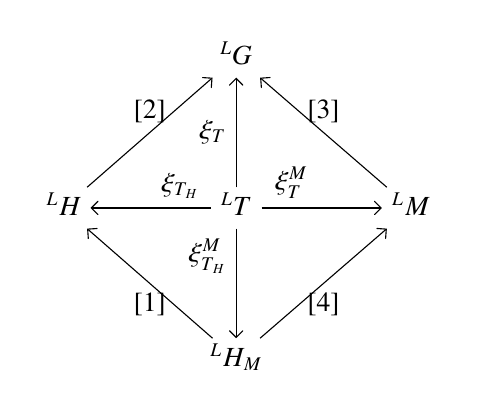
\begin{tikzpicture}[>=angle 90]
\matrix(a)[matrix of math nodes,
row sep=4em, column sep=4em,
text height=1.5ex, text depth=0.25ex]
{&{}^LG&\\
 {}^LH&{}^LT&{}^LM\\
 &{}^LH_M&\\};
\path[->](a-2-1) edge node[left,above]{[2]} (a-1-2);
\path[->](a-2-2) edge node[left]{$\xi_T$} (a-1-2);
\path[->](a-2-3) edge node[right,above]{[3]} (a-1-2);
\path[->](a-2-2) edge node[above,near start]{$\xi_{T_H}$} (a-2-1);
\path[->](a-2-2) edge node[left,above,near start]{$\xi_{T}^M$} (a-2-3);
\path[->](a-2-2) edge node[above,left,near start]{$\xi_{T_H}^M$} (a-3-2);
\path[->](a-3-2) edge node[left,below]{[1]} (a-2-1);
\path[->](a-3-2) edge node[right,below]{[4]} (a-2-3);
\end{tikzpicture}
\end{figure}


\noindent The triangles [1] and [3] as well as the outside square 
are commutative.
The triangles [2] and [4] fail to commute by the 
classes $a^G$ and $a^M$ respectively.  By the 
commutativity of [1], [3] and the outside square we have 
$a^G = a^M$ so that
$\Delta_{\text{III}_2}^M =\Delta_{\text{III}_2}^G$.
\end{proof}

\section{Homogeneity and General Descent} %10

We fix in this section an integer $Q$ satisfying $Q=p^\ell$, $\ell>0$, $Q\equiv 1
\mod c$, $c=c_G$.
We wish to compare the constants
$\Delta_0(\hgam,\ggam)$ and  $\Delta_0(\hgam^Q,\ggam^Q)$.
We assume in this section that
$(\hgam,\ggam)$ are matching strongly $G$-regular, strongly compact elements
such that $\hgam\in H(O_F)$,
$\ggam\in G(O_F)$.  
We also assume that the same $a$-data,
$\chi$-data, splitting, etc. are used for
$(\hgam,\ggam)$ and $(\hgam^Q,\ggam^Q)$.

First of all, $\Delta_{\text{I}}(\hgam,\ggam)=
\Delta_{\text{I}}(\hgam^Q,\ggam^Q)$
because this term depends on the above data and
Cartan subgroup $T_H,T$ and not directly on the 
elements $(\hgam,\ggam)$\ $(\hgam^Q,\ggam^Q)$.
Also $\Delta_{\text{III}_1}(\hgam,\ggam) =
\Delta_{\text{III}_1}(\hgam^Q,\ggam^Q)$
if we choose the element $h$, which enters into the
definition of this term, to be the same for
$(\hgam,\ggam)$ and $(\hgam^Q,\ggam^Q)$.

Write $\prod_{G/H}$ (resp. $\prod_{G/H}^{\circ}$) for the product of roots 
(resp. orbits of roots under the $T$-action of $\Gal(\overline F/F)$)
in $G$ but not $H$.  Define $\prod_{G/H}^\varep$, and $\prod_{G/H}^{\varep,\circ}$
similarly with respect to the roots in $G_\varep$ but not $H_\varep$.

\begin{cthm}{Lemma 10.1}  If $p>e_G+1$, 
$$
\begin{array}{lll}
\Delta_{\text{IV}}(\hgam^Q,\ggam^Q) 
&= |Q|^{m/2}\Delta_{\text{IV}}(\hgam,\ggam)=\\
\Delta_{\text{IV},\varep}
(\hgam^Q,\ggam^Q)
&=|Q|^{m/2}\Delta_{\text{IV},\varep}(\hgam,\ggam)
\end{array}
$$
where $m$ is the number of roots in $G_\varep$
but not in $H_\varep$ and $\varep$ is the absolutely semisimple part 
of $\ggam$.
\end{cthm}

\begin{proof}  $\Delta_{\text{IV}}(\hgam,\ggam)
=|\prod_{G/H}(\alpha(\gamma)-1)|^{1/2}$. If
$\gamma=\gamma_s\gamma_u$ topological Jordan decomposition
$$
\begin{array}{lll}
|\prod_\alpha(\alpha(\gamma)-1)|^{1/2}
&= |
\prod_{ \alpha(\gamma_s)\ne1}
(\alpha(\gamma_s)-1)|^{1/2}\quad
|\prod_{\alpha(\gamma_s)=1}
(\alpha(\gamma)-1)|^{1/2}\\
&=
|\prod_{G/H}^\varep(\alpha(\gamma)-1)|^{1/2}.
\end{array}
$$
Similarly, $\Delta_{\text{IV}}(\hgam^Q,\ggam^Q)=\Delta_{IV,\varep}
(\hgam^Q,\ggam^Q)$. If
$\alpha(\gamma_s)=1$ then by (3.1),
$|\alpha(\gamma)^Q-1|
=|Q||\alpha(\gamma)-1|$.
So
$\Delta_{IV,\varep}(\hgam^Q,\ggam^Q)
=|Q|^{m/2}\Delta_{\text{IV},\varep}(\hgam,\ggam)$.
\end{proof}

By (3.3), we may assume the $\chi$-data are selected to
be tamely ramified characters.

\begin{cthm}{Lemma 10.2}  If $p>e_G+1$,
$\Delta_{\text{II}}(\hgam^Q,\ggam^Q)=
\Delta_{\text{II}}(\hgam,\ggam)
\prod_{G/H}^{\varep,\circ}\chi_\alpha(Q)
$.
\end{cthm}

\begin{cthm}{Corollary 10.3}  Under the same conditions,
$
\Delta_{\text{II}}(\hgam^{Q^2},\ggam^{Q^2})
=\Delta_{\text{II}}(\hgam,\ggam)
$.
\end{cthm}

\begin{proof} $\chi_\alpha$ on $F_\pm\owns Q$
has order 2.
\end{proof}

\begin{proof}(Lemma).
$$
\frac{\Delta_{\text{II}}(\hgam^Q,\ggam^Q)}
     {\Delta_{\text{II}}(\hgam,\ggam)}
=\prod_\alpha^\circ\chi_\alpha\left(
\frac{\alpha(\gamma)^Q-1}
   {\alpha(\gamma)-1}
\right).
$$
If $\alpha(\gamma_s)\ne1$ then
$$
\frac{\alpha(\gamma)^Q-1}{\alpha(\gamma)-1}
=
\frac{1+x'_s(x_u^Q-1)}
     {1+x'_s(x_u-1)}$$
is topologically unipotent, where
$\alpha(\gamma)=x_sx_u$ is the topological Jordan 
decomposition of $\alpha(\gamma)$, and $x'_s = x_s/(x_s-1)$.
So 
$\chi_\alpha\left(\frac{\alpha(\gamma)^Q-1}
{\alpha(\gamma)-1}\right)=1$ if $\alpha(\gamma_s)\ne 1$.
So the product can be taken over roots in 
$G_{\varep}$ outside $H_{\varep}$.
If $\alpha(\gamma_s)=1$ we have by (3.1),
$\chi_\alpha\left(\frac{\alpha(\gamma)^Q-1}
{\alpha(\gamma)-1}\right)=\chi_\alpha(Q)$,
and the result follows.
\end{proof}

Before turning to the factor $\Delta_{\text{III}_2}$
we state a few preparatory lemmas.

\begin{cthm}{Lemma 10.4}  Suppose $p > e_G+1$.   If
$a^{2^r}$ is a tamely ramified character on $T(F)$ for some $r>0$ then $a$
is a tamely ramified character.
\end{cthm}

\begin{proof}  If $\reschar\ne 2$ every topologically unipotent
element is a square, and hence a $2^r$-power.  So if $\gamma$ is 
topologically unipotent, $\gamma=\delta^{2^r}$ for some $\delta$ and
$
\langle a,\gamma\rangle
= \langle a^{2^r},\delta\rangle=1.
$
\end{proof}

\begin{cthm}{Lemma 10.5} $r_q^2$ is independent of the gauge $q$.
\end{cthm}

\begin{proof}  $r_q = s_{q/p}r_p$ and $s_{q/p}^2 = 1$.
\cite{\LANGLANDSO, 2.4}.
\end{proof}

\begin{cthm}{Lemma 10.6}  $r_q^2$ is a cocycle.
\end{cthm}

\begin{proof}  The coboundary of $r_q$ is
$t_q$ and $t_q^2 = 1$ \cite{\LANGLANDSO,2.1.B,2.5.A}.
\end{proof}

Next we give an expression for the cocycle
$a(w) \in H^1(W_{E/F},\widehat T(\Com))$.
We add subscripts $G,H$ as needed to distinguish between
data for $G$  and $H$.  We also distinguish data by adding
a bar to data on $H$, e.g. $\overline r_p$. We use notation from \cite{\LANGLANDSO}.
$$
\begin{array}{lll}
\xi_T(w) &= r_p(w)n_G(\omega_T(\sigma))\times w,
     &\qquad w\mapsto \sigma\in \Gamma,\quad\xi_T:{}^LT\to {}^LG,\\
\xi_{T_H}(w) &=\overline r_p(w)n_H(\omega_{T_H}(\sigma))\times w,
	&\qquad \xi_{T_H}:{}^L{T_H}\to {}^LH,\\
\xi(w) &=m_0(\sigma)\times w, &\qquad \xi:{}^LH\to {}^LG.
\end{array}
$$
By definition, $a$ is given by
$$
\begin{array}{lll}
\xi\cdot\xi_{T_H}(w) =
\xi(\overline r_p(w)n_H(w_{T_H}(\sigma))\times w)
&=\overline r_p(w)n_H(w_{T_H}(\sigma))m_0(\sigma)\times w\\
&=a(w)r_p(w)n_G(\omega_T(\sigma)))\times w = a\cdot\xi_T(w).
\end{array}
$$
Define $\lambda_0$ by\quad
$m_0(\sigma)=\ {}^x\lambda_0(\sigma)n_G(\omega_H(\sigma))$, $x\Def \omega_{T_H}(\sigma)^{-1}$
where $\omega_H$ is defined by
$\omega_{T_H}(\sigma)\omega_H(\sigma)=
\omega_T(\sigma)$.
Then
$$
\begin{array}{lll}
\overline r_p(w)n_H(\omega_{T_H}(\sigma))\cdot{}^x\lambda_0(\sigma)
&=a(w)r_p(w)n_G(\omega_T(\sigma))n_G(\omega_H(\sigma))^{-1}\\
n_G(\omega_T(\sigma)) =n_G(\omega_{T_H}(\sigma)
\omega_H(\sigma)) &=
t_G(\omega_{T_H}(\sigma),\omega_H(\sigma))^{-1}
n_G(\omega_{T_H}(\sigma))n_G(\omega_H(\sigma)).
\end{array}
$$
So
$$
\overline r_p(w)\lambda_0(\sigma)n_H(\omega_{T_H}(\sigma))
= a(w)r_p(w)t_G(\omega_{T_H}(\sigma),
\omega_H(\sigma))^{-1}n_G(\omega_{T_H}(\sigma)).
$$
$$
a(w) =
\underbrace{\overline r_p(w)}_{\text{(1)}}
\underbrace{\lambda_0(\sigma)}_{\text{(2)}}
\underbrace{[n_H(\omega_{T_H}(\sigma))n_G^{-1}(\omega_{T_H}(\sigma))]}_{
\text{(3)}}
\underbrace{t_G(\omega_{T_H}(\sigma),\omega_H(\sigma))}_{\text{(4)}}
\underbrace{r_p(w)^{-1}}_{\text{(5)}}.
\taglet10.7
$$
Each of the bracketed terms lies in $\widehat T(\Com)$.

We will check that by raising $a$ to the fourth power,
the 3rd and 4th bracketed terms will become 1.
Also the remaining three terms $\overline r_p(w)$,
$\lambda_0(\sigma)$, $r_p(w)^{-1}$ will each be cocycles
when raised to the fourth power.


\begin{cthm}{Lemma 10.8}  $n_G(\omega_1\omega_2\cdots\omega_r)
= t\,n_G(\omega_1)\cdots n_G(\omega_r)$ for some $t=t(\omega_1,\ldots,\omega_r)$ satisfying 
$t^2 = 1$.
\end{cthm}

\begin{proof}  Clear from \cite{\LANGLANDSO,2.1.A}.
\end{proof}

By \cite{\DERIZIOTIS} we may assume that the simple roots 
of $\what H$ are a subset of the extended set of simple roots $\Delta\cup\{-r_0\}=
\tild\Delta$ of $\what G$.

\begin{cthm}{Lemma 10.9}  There is a choice of root vectors  $X_\alpha^H$,
$X_\alpha^G$ such that 
{\rm(i)} $n_G(\omega_\alpha) = n_H(\omega_\alpha)$ if
$\alpha$ is a simple root of $H$ in $\Delta$.
{\rm(ii)}  $n_G(\omega_{-r_0}) = t_0n_H(\omega_{-r_0})$
where $t_0^4 = 1$.
\end{cthm}

\begin{proof}  The first statement is obvious by definition
if the root vectors are chosen to be the same: 
$X_\alpha^H=X_\alpha^G$, $\alpha\in\Delta$.  Define $t_0$ by 
$n_G(\omega_{-r_0}) = t_0n_H(\omega_{-r_0})$.  Set
$\omega = \omega_{-r_0}$.
$$
n_G(\omega)^2 = t_G(\omega,\omega) =
t_0^\omega t_0n_H^2(\omega_{-r_0})
= t_0^\omega t_0t_H(\omega,\omega).
$$                                                      
We are still allowed to pick $X_-$ the simple root 
vector associated to $-r_0$.
Allowing a momentary conflict in the meaning of $H$, we
let $\varphi:SL_2\to \what H$ be attached to the Lie triple 
$\{X_{-r_0}=X_-$, $X_+$ and coroot $H\}$, and set  
$T_0 = 
\{x\in T\suchthat \alpha_{-r_0}(x) = 1\}$.
Let $M_0$ be the Levi factor such that
$M_0 =T_0\varphi(SL_2)$.
We select $X_-$ so that
$n_G(\omega_{-r_0})n_H(\omega_{-r_0})^{-1} = 
t_0 \in T_0$.  This is always possible by the 
$2\times2$ calculation:
$$
\begin{pmatrix} 0&t\\-t^{-1}&0\end{pmatrix}
\begin{pmatrix} 1&x\\0&1\end{pmatrix}
\begin{pmatrix} 1&0\\-1/x&1\end{pmatrix}
\begin{pmatrix} 1&x\\0&1\end{pmatrix}
%=
%\begin{pmatrix} 0&t\\-t^{-1}&0\end{pmatrix}
%\begin{pmatrix} 0&x\\-x^{-1}\end{pmatrix}
=\begin{pmatrix} -t/x&0\\0&-x/t\end{pmatrix}.
$$
Then $t_0^\omega t_0 = t_0^2 = t_G(\omega,\omega)/t_H(\omega,\omega)$, which
has order 2.
\end{proof}

\begin{cthm}{Corollary 10.10}  $a^4= \overline r_p^4 \lambda_0^4/r_p^4$.
\end{cthm}

\begin{proof}  By (10.8), (10.9) The 4th powers of the terms 
$n_H(\omega_{T_H}(\sigma))n_G^{-1}(\omega_{T_H}(\sigma))$
and $t(\omega_{T_H}(\sigma),\omega_H(\sigma))$ in (10.7) are 1.
\end{proof}

\begin{cthm}{Corollary 10.11}  $\lambda_0^4$ is a cocycle.
\end{cthm}

\begin{proof}  The other terms of (10.10) are.
\end{proof}

\begin{cthm}{Remark 10.12}  $(\overline r_p/r_p)^2$
is independent of the choice of $\xi:{}^LH\to {}^LG$.
\end{cthm}

\begin{cthm}{Lemma 10.13}  $\lambda_0^4$ depends on $T_H$ only through $H$.
\end{cthm}

\begin{proof}  
Write $\lambda_0^4 = \lambda_{T_H}$ to make the possible dependence on $T_H$
explicit.
$$\lambda_{T_H}(\sigma) = {}^{\omega_{T_H}(\sigma)}\left[m_0(\sigma)n_G(\omega_H(\sigma))\right]^4.$$
Since $\lambda_{T_H}$ is a cocycle, 
$\lambda_{T_H}(\sigma)^{-1} = \sigma(\lambda_{T_H}(\sigma^{-1}))$.  Hence
$$\lambda_{T_H}(\sigma)^{-1}= {}^{(\omega_T(\sigma)\rtimes \sigma)\omega_{T_H}(\sigma^{-1})}
  \left[m_0(\sigma^{-1})n_G(\omega_H(\sigma^{-1}))\right]^4.$$
But since $\Gamma \to\Omega\rtimes\Gamma$, $\sigma\mapsto \omega_T(\sigma)\rtimes \sigma$ is
a homomorphism we have
$$\begin{array}{lll}
	(\omega_T(\sigma)\rtimes \sigma)\omega_{T_H}(\sigma^{-1}) &=
	(\omega_T(\sigma)\rtimes \sigma)\omega_T(\sigma^{-1})\omega_H(\sigma^{-1})^{-1} \\
	&=
	(\omega_T(\sigma)\rtimes \sigma)(\omega_T(\sigma^{-1})\rtimes \sigma^{-1})(1\rtimes \sigma)
		\omega_H(\sigma^{-1})^{-1} \\ &=
	(1\rtimes\sigma)(\omega_H(\sigma^{-1})^{-1})\end{array}
$$
which is independent of $T_H$. Hence $\lambda_{T_H}$ is independent of $T_H$.
\end{proof}

\begin{cthm}{Corollary 10.14}  $\lambda_0^4$ gives an unramified
character on the maximally split Cartan subgroup $\Bbb T_H(F)$ of $H$.
\end{cthm}

\begin{proof}  The cocycle $\lambda_0^4$ of the Weil group is
clearly the inflation of a cocycle on $\Gal(E/F)$ for an
appropriate unramified extension $E/F$ because both $\omega_H(\sigma)$
and $m_0(\sigma)$ factor through an unramified extension.  By \cite{\LABESSEC},
 such cocycles correspond to unramified
characters on the $\Bbb T_H(F)$.  
\end{proof}

\begin{cthm}{Proposition 10.15}  If the $\chi$-data is 
tamely ramified then the character
$\langle a,\gamma\rangle$ given in the term 
$\Delta_{III_2}$ is also  tamely ramified.
(As always $\reschar \ne 2$.)
\end{cthm}

\begin{proof}  By the construction of Labesse, it is 
enough to show that $a^4\in H^1(W_{E/F},\widehat T(\Com))$
is the corestriction of a  tamely ramified character
$\varphi\in\Hom_c(E^\times,\widehat T(\Com))$.  This follows
immediately from the following lemma and (10.10), (10.14).
\end{proof}

Extend each character $\chi_\lambda$ to a tamely ramified character $\chi_{\lambda,E}$
on $E^\times$.  Then
define 
$\varphi_\lambda\in \Hom_c(E^\times,\widehat T)$ by
$\varphi_\lambda(u) = \chi_{\lambda,E}(u)^\lambda$.

\begin{cthm}{Lemma 10.16}  
$\operatorname{Cor}\left[\prod_{G/H}^\circ\varphi_\lambda\right]$
is cohomologous to $r_p^2/\overline r_p^2$.
\end{cthm}

\begin{proof}  $r_p$ itself is a product of terms $r_p^\lambda$ indexed by orbits
of roots $\lambda$. 
If $\chi_\lambda$ is a character on $F_+^\times$ we may view it as
a character $\widehat \chi_\lambda$ on $W_{E/F_+}$ by local
class field theory. By Section 5 applied to the split rank-one torus, 
this identification is given by
$$
\chi_\lambda\mapsto \widehat\chi_\lambda =\operatorname{Cor}'_{E/F_+}\chi_{\lambda,E}.
$$
where $\operatorname{Cor}'_{E/F_+}$ is the corestriction from $\Hom_c(E^\times,\Bbb C^\times)$ to 
$H^1_c(W_{E/F_+},\Bbb C^\times)$.  Let $\operatorname{Cor}_+$ be the corestriction
map associated to $W_{E/F_+}\to W_{E/F}$. 
Since $\Gal(E/F_+)$ acts trivially on $\lambda$,
we have
$\operatorname{Cor}_{E/F}\varphi_\lambda
=\operatorname{Cor}_{+}\left[
\operatorname{Cor}'_{E/F_+}{\chi_{\lambda,E}}^\lambda\right]
=\operatorname{Cor}_{+}(\widehat\chi_\lambda^\lambda)$
which we will now show to be equal to $r_p^{\lambda}(w)^2$. 

We recall
the definition of $r_p^{\lambda}(w)$.
Fix representatives $\{\tau_p\}$
in $\Gamma$ for $\Gamma/\Gamma_\pm$.  Fix 
$a,b$ in $\Gamma_{\pm}\subseteq\Gamma$ trivial and nontrivial
respectively in $\Gamma_\pm/\Gamma_+$.  Set 
$ R^+ = R^+_p=\{a\tau_p\}$, $R^- = R^-_p = \{b\tau_p\}$.
Then fixing appropriate representatives $w_\tau$ in $W$ for elements of $R^+$,
$R^-$,
$$
r_p^{\lambda}(w)\Def
\prod_{\tau\in R^+}\widehat\chi_\lambda(w_\tau ww_\sigma^{-1})^{
w_\tau^{-1}\lambda}
$$
where $\sigma\in R^+\cup R^-$ is defined by
$w_\tau ww_\sigma^{-1}\in W_{E/F_+}$.  Now we change 
the set
of representatives to $\tau_q=a^{-1}b\tau_p$.
So $R^+_q = R^-_p$, $R^-_q=R^+_p$.
The gauge for this data is $q= -p$.  This gives
$$
r_{-p}^{\lambda}(w) =\prod_{R^+_q}
\widehat\chi_\lambda(w_\tau ww_\sigma^{-1})^{
w_\tau^{-1}\lambda}
=\prod_{R^-_p}\widehat \chi_\lambda(
w_\tau ww_\sigma^{-1})^{w_\tau^{-1}\lambda}.
$$
Now
$$
r_p^{\lambda}r_{-p}^{\lambda}
=\prod_{R^+\cup R^-}(\cdots)
=\operatorname{Cor}_{+}\widehat\chi_\lambda^\lambda
=\operatorname{Cor}_{E/F}\varphi_\lambda.
$$
Also $r_{-p}=s_{-p/p}r_p$
and $s_{-p/p} = 1$ (\cite{\LANGLANDSO, 2.4}).
The result follows.
\end{proof}

Now finally, we turn to $\Delta_{III_2}(\gamma_H,\gamma_G)$
and the completion of the results of this section.

\begin{cthm}{Theorem 10.17}  For $p>e_G+1$ 
and $\gamma_H,\gamma_G$
strongly compact
$$
\Delta_0(\gamma_H^{Q^2},\gamma_G^{Q^2})
=|Q|^m\Delta_0(\gamma_H,\gamma_G)
$$
where $m$ is the number of roots outside $H_{\varep}$
but in $G_{\varep}$.
\end{cthm}

\begin{proof} By the preceding results, it is enough
to check that 
$\Delta_{\text{III}_2}(\gamma_H^Q,\gamma_G^Q)
= \Delta_{\text{III}_2}(\gamma_H,\gamma_G)$
But
$$
\begin{array}{lll}
\Delta_{\text{III}_2}(\gamma_H,\gamma_G)
&\Def
\langle a,\gamma\rangle =\langle a,\gamma_s\rangle
\langle a,\gamma_u\rangle = \langle a,\gamma_s\rangle\\
&=\langle a,\gamma_s^Q\rangle =\langle a,\gamma_s^Q\rangle
\langle a,\gamma_u^Q\rangle = \langle a,\gamma^Q\rangle\\
&=\Delta_{\text{III}_2}(\gamma_H^Q,\gamma_G^Q)
\end{array}
$$
since $\gamma_s^Q=\gamma_s$ and $a$ is tamely ramified by (10.15).
\end{proof}

\begin{cthm}{Theorem 10.18}  For $p > e_G+1$, $\Delta_0(\gamma_H,
\gamma_G) = \Delta_{0,\varep}(	\gamma_H,\gamma_G)$.
\end{cthm}

\begin{proof} $\Delta_0(\gamma_H,\gamma_G) =
{\Delta_0(\gamma_H^{Q^2},\gamma_G^{Q^2})}/{|Q|^m}$.
As $Q\to\infty$, $\gamma_H^Q\to \gamma_{H,s}$,
$\gamma_G^Q\to \gamma_{G,s}$ and we have seen
$\Delta_0(\gamma_H^Q,\gamma_G^Q) =\Delta_{0,\varep}(\gamma_H^Q,\gamma_G^Q)$
near $\gamma_{H,s}$, $\gamma_{G,s}$.  Also
$\Delta_{0,\varep}(\gamma_H,\gamma_G)
={\Delta_{0,\varep}(\gamma_H^{Q^2},\gamma_G^{Q^2})}/{|Q|^m}$
which equals
${\Delta_0(\gamma_H^{Q^2},\gamma_G^{Q^2})}/{|Q|^m}
= \Delta_0(\gamma_H,\gamma_G)$.  Here $\varep$ is the absolute 
semisimple part of $\gamma_G$ (or $\gamma_H$).
\end{proof}




\section{Central Characters} %11

We identify $Z^0 = Z^0_G$ canonically with a subgroup of
$Z_H$.
\begin{cthm}{Lemma 11.1} For $z\in Z^0$, we have $\Delta(z\hgam,z\ggam)
=\langle a,z\rangle\Delta(\hgam,\ggam)$,
 where $a\in H^1(W_F,\widehat T(\Com))$ is computed
relative to any $\hgam,T_H\to T$, etc.
\end{cthm}

\begin{proof}  \cite{\LANGLANDSO}.\end{proof}

\begin{cthm}{Lemma 11.2}  $\langle a,\cdot \rangle$ is an unramified
character on every unramified Cartan subgroup $T_H$ of $H$.\end{cthm}

\begin{proof}  %By (11.1) we may 
%compute $\langle a,z\rangle$  using the maximally split Cartan subgroup of $H$. 
Referring to the definition of the cocycle $a$, and
using \cite{\LANGLANDSO, 2.1.A}, together with $\omega_{T_H}(\sigma)=1$, the
cocycle $a$ becomes
$$
a(w) = \overline r_p(w)m_0(\sigma)n_G(\omega_H(\sigma))^{-1}r_p(w)^{-1}.
$$
Select the $\chi$-data to be unramified.
Let $E/F$ be an unramified extension splitting $T_H$.  By
the criterion of Labesse \cite{\LABESSEC,6.3,5.9}, $\langle a,\cdot\rangle$
is unramified on $T_H(F)$ if $a$ is represented by a cocycle
in $Z_c^1(W_{E/F},\what T_H)$ which is trivial on the units of $E^\times
\subset W_{E/F}$.  On $E^\times$, $a(x)$ reduces further to
$$a(x) = \overline r_p(x) r_p(x)^{-1}.$$
By Langlands and Shelstad \cite{\LANGLANDSO,p237}, the restriction
of $r_p =\prod r_p^\lambda$ to $E^\times$ is given by
$$r_p^\lambda(x) = \prod_{i=1}^n\chi_\lambda(\text{Nm}^E_{F_+}
	\sigma_ix)^{\sigma_i^{-1}\lambda},\ \ x\in E^\times,$$
and a similar formula holds for $\overline r_p$.  Since $\chi_\lambda$ is
unramified, it is now clear that $a(x)$ restricted to units of
$E^\times$ is trivial.
\end{proof}

%\cite{\LABESSEC, 5.9} or Section 10 shows that $\overline r_p$,
%$r_p$ are inflated from cocycles in
%$H^1(\Gal(E/F),\widehat T)$, $E/F$ unramified.  Hence $a(w)$ itself is inflated
%from a cocycle of some $H^1(\Gal(E/F),\widehat T)$, $E/F$ unramified.

%Set $\what S\Def\what G/(\what G)_{der}
%=\what T_H/\what T_{der}
%\qquad
%\what T_{der} =\what T_H\cap(\what G)_{der}$

%\begin{cthm}{Lemma 11.2}  If $a_1,a_2$ are unramified 
%cocycles in $H^1(W_{E/F},\what T)$ with
%equal images in $H^1(W_{E/F},\what S)$, then
%they are equal in $H^1(W_{E/F},\what Z_G)$.
%\end{cthm}

%\begin{proof} Let $\what G$  be a semisimple group with $L$-group
%$\what G_{der}$, and let $\tild T$ be a torus in
%$\tild G$ corresponding to $\what T_{der}$.  Suppose $a$
%is an unramified cocycle of $H^1(W_{E/F},\what T_H)$ with trivial
%image in $H^1(W_{W/F},\what S)$.  Then the exact sequence
%$$
%H^1(W_{E/F},\what T_{der})
%\to H^1(W_{E/F},\what T_H)
%\to H^1(W_{E/F},\what S)
%$$
%%shows that $a$ is the image of some unramified cocycle
%$b$ in $H^1(W_{E/F},\what T_{der})$.  By abelian class field theory
%this shows that the character $\theta$ on $T_H(F)$ associated to $a$ is
%obtained pulling back an unramified character on
%$\tild H(F)$ by the map $T_H @>>i>\tild T$ dual to 
%$\tild T_{der} \subseteq \what T_H$.  In particular,
%$\theta$ is trivial on 
%$Z_G(F)\subseteq i^{-1}(Z_{\tild G}(F))\subseteq i^{-1}(\tild T(O_F))$.
%So dually $a$ is trivial in $H^1(W_{E/F},\what Z_G)$.
%\end{proof}

%Denote the projection $\what T\to\what S$ by $\delta$.
%$$
%\delta\, a(w) = \delta\, m_0(\sigma)\in\what S
%$$
%because by construction
%$\overline r_o(w), r_p(w), n_G(\omega_H(\sigma))$ all lie in the
%derived group $\what G_{der}$

To identify the unramified character $\langle a,z\rangle$ in terms suitable
for application to endoscopy we recall some well-known constructions
found in \cite{\BOREL},\cite{\MACDONALD}.   Adopt the notation
of \cite{\BOREL}, adding subscripts $G$ and $H$ to distinguish
data on $\what G$ and $\what H$.  There is a canonical surjection
$\what T_G\to \what Y_G$ inducing bijections
$$\what Y_G/{}_kW_G \bij (\what T_G\rtimes\sigma)/\text{int}\,{}_k\what N
	\bij (\what G\rtimes\sigma)_{ss}/\text{int}\,\what G.$$
Similar bijections hold with $G$ replaced by $H$.
Using $\xi:{}^LH\to{}^LG$ and the bijections above, functions on 
$\what Y_G/{}_kW_G$ pull back by $\xi^*$ to functions on $\what Y_H/{}_kW_H$.
Let $s_H$ and $s_G$ be matching elements in $\what Y_H$ and $\what Y_G$ by 
these bijections, and let $t_H$ and $t_G$ be corresponding lifts to 
$\what T_H$ and $\what T_G$.  By construction $\xi(t_H\rtimes\sigma) =
t_Hm_0(\sigma)\rtimes\sigma\in {}^LG$ is $\what G$-conjugate to $t_G\rtimes\sigma
\in \what T_G\rtimes \sigma$.  The spherical measures $\what \omega_s$ attached
to $s\in \what Y_G$ identifies the Hecke algebra $H(G)$ on $G$ with coordinate
functions on $\what Y_G/{}_kW_G$ by
$$f: s\to \what\omega_s(f).$$
By these identifications $\xi^*$ induces a map from the Hecke algebra of $G$
to that of $H$, which we denote $\mathcal{ H}:H(G)\to H(H)$.

Let $\Bbb T_d$ denote the maximal split subtorus of $\Bbb T_G$.
Then $\what Y_G$ is canonically identified with the group of
unramified characters on $\Bbb T_G$ giving a pairing
$\what Y_G \times \Bbb T_G(F) \to^{\langle,\rangle} \Bbb C^\times$.
Pick $z\in \Bbb T_d(F) \cap Z_G^0$.  
Define $R^G_z$ for $z\in Z_G(F)$ by $(R^G_zf)(x) = f(xz)$, and
define $R_z^H$ analogously on $C_c^\infty(H)$.

\begin{cthm}{Lemma 11.3}  For $z\in\Bbb T_d(F) \cap Z_G^0$,
we have $R_z^H\mathcal{ H}(f) = \langle a,z\rangle\mathcal{ H}(R_z^Gf)$.
\end{cthm}

\begin{proof}
Tracing the identifications through using \cite{\MACDONALD}
one easily checks that $\what\omega_s^G(R_z^Gf) = \langle s,z^{-1}\rangle
\what\omega_s^G(f)$, $s\in \what Y_G$, $f\in H(G)$.  A similar
formula holds on the Hecke algebra of $H$.

Now if $s_H$ and $s_G$ in $\what Y_H$ and $\what Y_G$ correspond
by $\xi$, and if $s\in Z_G^0\cap \Bbb T_d(F)$, then
$$\what\omega^H_{s_H}(\mathcal{ HR}_z^Gf) = 
  \what\omega_{s_G}^G(R_z^Gf) = \langle s_G,z^{-1}\rangle \what\omega^G_{s_G}(f) =
  \langle s_G,z^{-1}\rangle \what\omega_{s_H}^H(\mathcal{ Hf}),$$
$$\what\omega_{s_H}^H(R_z^H\mathcal{ Hf}) = \langle s_H,z^{-1}\rangle
	\what\omega_{s_H}^H(\mathcal{ Hf}).$$
Hence
$$\langle s_G,z\rangle\what\omega_{s_H}^H(\mathcal{ HR}_z^Gf) =
	\langle s_H,z\rangle \omega_{s_H}^H(R_z^H\mathcal{ Hf}).$$
Now we will show below that (*)\ $\langle s_G,z\rangle\langle s_H,z^{-1}\rangle
	= \langle a,z\rangle$.
Hence 
$$\what\omega_{s_H}^H(\langle a,z\rangle \mathcal{ HR}_z^Gf) = 
	\what\omega^H_{s_H}(R_z^H\mathcal{ Hf})$$
for all $s_H\in \what Y_H$.  Thus $\langle a,z\rangle \mathcal{ H}(R^G_zf)
	=R_z^H\mathcal{ H}(f)$.

Finally we return to the identity (*).  Place a subscript ``$un$''
to denote unramified classes in $H^1$.
Let $a_G,a_H\in H^1_{un}(W_{E/F},\what T)$ represent $t_G\rtimes\sigma,
t_H\rtimes\sigma$ respectively.  We must show $a_Ga_H^{-1}a^{-1}$
has trivial image in $H^1_{un}(W_{E/F},\what Z_G)$.  Let $\what G_{der}$ denote
the derived subgroup of $\what G$, and set $\what T_{der} = \what T\cap
\what G_{der}$.  It is easily checked that the composite
$$H^1_{un}(W_{E/F},\what T_{der}) \to H^1_{un}(W_{E/F},\what T) \to
  H^1_{un}(W_{E/F},\what Z_G)$$
is zero.  Hence $a_Ga_H^{-1}a^{-1}$ has trivial image in $H^1_{un}(W_{E/F},\what Z_G)$
if its image in $H^1_{un}(W_{E/F},\what T/\what T_{der}) =
H^1_{un}(W_{E/F},\what G/\what G_{der})$ is trivial.
Now by definition $t_G$ is $\sigma$-conjugate to $t_Hm_0(\sigma)$,
$(t_G = x^{-1}t_Hm_0(\sigma)\sigma(x))$ so that $t_G$ and $t_Hm_0(\sigma)$
lead to the same class in $H^1_{un}(W_{E/F},\what G/\what G_{der})$.
But the product of $t_H$ with $a(w) = \overline r_p(w) m_0(\sigma) 
n_G(\omega_H(\sigma))^{-1} r_p(w)^{-1}$ is clearly equal to
$t_Hm_0(\sigma)$ modulo $\what G_{der}$ (which contains $\overline r_p$,
$r_p$, $n_G$).  Hence $a_G = a_Ha$ in $H^1_{un}(W_{E/F},\what Z_G)$.
\end{proof}

\vfil\eject
\centerline{\bf PART III.  ORBITAL INTEGRALS}\vskip3pc
\section{Harish-Chandra Descent} %12

Suppose we have a commutative diagram
$$
\begin{CD}
{}^LH @>\xi>> {}^LG\\
@AAA  @AAA\\
{}^L{H_M} @>{\xi_M}>> {}^LM
\end{CD}
$$
where $M$ is a Levi factor of a parabolic subgroup 
of $G$.  Let $\mathcal{ H}_B^A$ be the map from the Hecke algebra of A to the Hecke algebra
of $B$ corresponding to ${}^LA\to {}^LB$.  Then
$\mathcal{ H}_{H_M}^M\mathcal{ H}_{M}^G=\mathcal{ H}_{H_M}^H\mathcal{ H}_H^G$. 
By Harish-Chandra descent and induction on groups of
smaller rank, for suitable elements
$(\hgam,\ggam)\in H_M\times M$ (using 9.2)
$$
\begin{array}{lll}
\sum \Delta_0(\hgam,\ggam)\Phi_{T,G}(\ggam,f)
&=\sum\Delta_0^M(\hgam,\ggam)\prod_{H/H_M}|1-\alpha(\gamma)|^{-1/2}\Phi_{T,M}
       (\ggam,\mathcal{ H}_M^G(f))\\
&=\prod_{H/H_M}|1-\alpha(\gamma)|^{-1/2}\Phi_{T,H_M}^{st}(\ggam,\mathcal{ H}_{H_M}^M\mathcal{ H}_M^G(f))\\
&=\prod_{H/H_M}|1-\alpha(\gamma)|^{-1/2}\Phi_{T,H_M}^{st}(\ggam,\mathcal{ H}_{H_M}^H\mathcal{ H}_H^G(f))\\
&=\Phi_{T,H}^{st}(\ggam,\mathcal{ H}_H^G(f)).
\end{array}
$$
So the fundamental lemma in general follows from the fundamental lemma for
compact elements.  So it is enough to consider compact elements.

Suppose $z\in Z_G^0(F)$,
and suppose the matching is known for $\hgam$.
Then using (11.1) and (11.3)
$$
\begin{array}{lll}
\sum_{\ggam}\Delta(z\hgam,z\ggam)\Phi_T(z\ggam,f)
&=\sum_{\ggam}\langle a,z\rangle
\Delta(\hgam,\ggam)\Phi(\ggam,R_z^Gf)\\
&=\langle a,z\rangle\Phi_{T,H}^{st}(\hgam,\mathcal{ H}(R_z^Gf)) \\
&=\Phi_{T,H}^{st}(\hgam,\langle a,z\rangle\mathcal{ H}(R_z^Gf))\\
&=\Phi_{T,H}^{st}(\hgam,R_z^H\mathcal{ H}(f))\\
&=\Phi_{T,H}^{st}(z\hgam,\mathcal{ H}(f)).
\end{array}
$$
So the fundamental lemma follows
for $z\hgam$ from the 
fundamental lemma for $\hgam$. 

\vskip3pc
\section{Descent for Absolutely Semisimple Elements} %13

We will apply descent arguments to $\gamma=\gamma_s\gamma_u$
noting that every element is either topologically unipotent ($\gamma_s=1$) 
or contained in the centralizer $C_G(\gamma_s)^0$
of a nontrivial semisimple element.  The following version of Kazhdan's lemma,
found in
Kottwitz \cite{\KOTTWITZS}, is essential. 
\begin{cthm}{Lemma 13.1}  Let $\varepsilon\in G(O_F)$ be
absolutely semisimple. Then $G_{\varepsilon}$ is quasi-split
and splits over an unramified extension.  Also $G_{\varepsilon}$
is naturally defined over $O_F$ as well as the inclusion $G_\varepsilon\subseteq G$.
$G_{\varepsilon}(O_F)$ is hyperspecial.  Finally, if $\varepsilon^h\in G(O_F)$ then
$h\in G_\varepsilon(\overline F) G(O_F)$.
\end{cthm}

Let $\gamma\in G(O_F)$ be a strongly
regular element with absolutely semisimple part $\varepsilon$.  
We consider $\kappa$-orbital integrals:
$$
\Phi_{T,G}^\kappa(\gamma,f)
=\int_{(T\backslash G)(F)}
\kappa(\sigma(g)g^{-1})
f(g^{-1}\gamma g)d\dot g.
$$
Suppose that $dt$ and $dg$ are invariant measures on $G$
(arising as usual from an invariant form) and that
$dt\ d\dot g = dg$. Set
$f_1=\frac{\Char G(O_F)}{\Vol(G(O_F),dg)}$.
Let $dh$ be an invariant measure on $G_{\varepsilon}$, and suppose
that $dt\ d\dot h = dh$ (same $dt$ as above). Set
$f_2=\frac{\Char G_{\varepsilon}(O_F)}{\Vol(G_{\varepsilon}(O_F),dh)}$.
Let $\kappa_\varepsilon$ be the restriction of $\kappa$ to $G_\varepsilon$.  Then
\begin{cthm}{Lemma 13.2}  Under the assumptions given above,
$$
\Phi_{T,G}^\kappa(\gamma,f_1) = \Phi_{T,G_\varepsilon}^{\kappa_\varepsilon}(\gamma,f_2).
$$
\end{cthm}

\begin{proof}  Same as \cite{\HALESU}, replacing Kazhdan's lemma by (13.1).
\end{proof}

Combined with (10.18), this shows that the fundamental lemma for the identity of the
Hecke algebra follows from the fundamental lemma for topologically unipotent elements.

\vskip3pc
\section{Regular Unipotent Orbital Integrals} %14

It can be easily seen that the canonical normalization of transfer factors is the
correct normalization for the fundamental lemma by comparing the orbital integrals
of strongly regular absolutely semisimple elements.   This section shows that
a much stronger compatibility condition holds for the transfer factors: the first
term of the asymptotic expansion (Shalika germ expansion) for the $\kappa$-orbital integral
of $G$ with transfer factor, coincides with the first term of the first term of the
asymptotic expansion on $H$.  By results of Shelstad \cite{\SHELSTAD} the germ is
either 1 or 0.  So to check that the first term of the expansions coincide it is
enough to compute and compare the unipotent regular orbital integrals for $G$ and $H$.
This computation is carried out in this section.   When $G$ and $H$ split over the
same unramified extension, descent properties for the maximally split Cartan subgroup of $G$
give the comparison by trivial arguments.  
When $G$ and $H$ split over different extensions more work
is required.  We make use of the results of Section 4 to reduce to a small number
of cases.

Let $\kappa$ be the character of $H^1(\Gal(E/F),\Bbb T_H)$ defining the
endoscopic group $H$ of $G$.  Then $\kappa$ defines \cite{\HALEST,VI-2} %thesis VI-2
for each simple
root $\alpha$ a character $\kappa^\alpha:F_\alpha\to\Com^\times$
where $F_\alpha$ is the field extension of $F$ over which
the root $\alpha$ becomes fixed by the Galois group.
We recall the definition.  We have a sequence
\begin{align*}
\begin{CD}
F^\alpha
@>{\varphi_\alpha}>>
\Bbb T_{G,\adj}(F) @>>>
\Bbb T_{G,\adj}(F)/\Bbb T_G(F)
\end{CD}\qquad\qquad\qquad\qquad\qquad\qquad\\
\begin{CD}
\text{}\qquad\qquad @>\delta>>
H^1(\Gal(E/F),Z_G)
@>>>
H^1(\Gal(E/F),\Bbb T_H)
@>\kappa>> \Com^\times.
\end{CD}
\end{align*}
The composite of these maps is $\kappa^\alpha$.  Here
$\varphi_\alpha$ is defined by
$$
\beta(\varphi_\alpha(x)) =
\begin{cases}
\sigma x &\text{\ if\ } \beta=\sigma\alpha\ \ \sigma\in\Gal(F_\alpha/F)\ \ 
\text{\ for all roots\ }  \beta \text{\ of\ } \Bbb T_G.\\
1 &\text{otherwise}.
\end{cases}
$$
It follows from the work of Langlands and Shelstad that
the orbital integral on the
stable class of regular unipotent elements that arises
as the coefficient of the regular germ of a $\kappa$-orbital 
integral is
$$
f\mapsto
\mu_{reg}^\kappa(f) =
\int_{\overline N}\int_N
m_\kappa(n)f(n^{\overline n})dnd\overline n
$$
where $f\in C_c^\infty(G)$, $N$ unipotent radical of 
$\Bbb B$, $\overline N$ unipotent radical of
the Borel subgroup opposite $\Bbb B$ through $\Bbb T_G$.
$m_\kappa(n)\Def\prod_\CurlyS\kappa^\alpha(x_\alpha)$ where
$n=\prod_{\beta>0}\exp(x_\beta X_\beta)$
and the product $\prod_\CurlyS$ runs over the set $\CurlyS$ of
$\Gal(\overline F/F)$-orbits of simple roots.
Also $dn, d\overline n$ are Haar measures on 
$N,\overline N$ obtained as a product of Haar measures
$dx_\beta$ ($\beta$ roots) normalized so that
$\int_{O_{F_\beta}}dx_\beta = 1$.  Another expression for this
integral is \cite{\HOWE}
$$
f\to \mu_{reg}^\kappa(f)
= c\int_K\int_N
f(n^k)m_\kappa(n)dn\,dk\quad
$$
for some constant $c$ independent of $\kappa$ and $f$.  It is this
latter integral that we will compute on the
characteristic function of $K\Def G(O_F)$ to obtain
$$
\mu_{reg}^\kappa(f) = c\int_{N\cap K}
m_\kappa(n)dn\Vol(K,dk)
=c\{\prod_\CurlyS\int_{O_{F_\alpha}}
\kappa^\alpha(x_\alpha)dx_\alpha\}\Vol (K,dk).
$$
Since $\Bbb T_H$ is unramified,  a prime
$\pi$ of $O_F$ is also prime in $O_{F_\alpha}$.
If we set $\kappa^\alpha(\pi)=\zeta_\alpha$, and set
$q_\alpha=q^{[F_\alpha:F]}$ then
$$
\mu_{\operatorname{reg}}^\kappa(\Char(K))/{\Vol(K,dk)}
= c\prod_\CurlyS\left(1-\frac1{q_\alpha}\right)
\left(
1+\frac{\zeta_\alpha}{q_\alpha}
+\frac{\zeta_\alpha^2}{q_\alpha^2}
+\cdots\right)
= c\prod_\CurlyS
\frac{(1-\frac1{q_\alpha})}
     {(1-\frac{\zeta_\alpha}{q_\alpha})}.
$$
To compute $c$ we set 
$\kappa=1$.  Then 
$\mu_{\reg}^{st}(f) = c\cdot\iint f(n^k)dndk$.
Set $f$ equal to the characteristic function
of $\{n^{\overline n}\suchthat
n\in N\cap K, \overline n \in \overline N\cap K\}$.
For any unramified group $G$ over $O_F$ set $[G]\Def |G(\Bbb F_q)|/q^{\dim\, G}$.
Then integrating $f$ as in \cite{{\HALESU,\HALESO}} we obtain:

%Then
%$\mu_{\reg}^{st}(f) = 1$ and if 
%$n^k\in X$ then $n\in K\cap N$,
%$k\in (B_0\cap K)(\overline N\cap K)$.
%So
%$$
%\int f(n^k)dndk =\Vol[(B_0\cap K)(\overline N\cap K,dk)]
%= \frac{\#\tild B_0\#\tild N}
%        {\#\tild G}\Vol(K,dk).
%$$
%Thus
%$$
%c =\frac{\#\tild G}{\#\tild B_0\#\tild N\Vol(K,dk)}.
%$$
%Thus we have proved:

\begin{cthm}{Lemma 14.1}
$$
\mu_{\reg}^\kappa(\Char(K))=
\frac{|\tild G|}{|\tild B||\tild N|}
\prod_\CurlyS
\frac{
(1-\frac1{q_\alpha})}
{(1-\frac{\zeta_\alpha}{q_\alpha})}
= \frac{[G]}{[\Bbb T_G]}
\prod_\CurlyS
\frac{
(q_\alpha-1)}
{(q_\alpha-\zeta_\alpha)}.
$$
\end{cthm}

Set $1_G={\Char(G(O_F))}/{[G]}$ for any
unramified group $G$ over $O_F$.  The main result of this section
is

\begin{cthm}{Proposition 14.2} $\mu_{\reg}^\kappa(1_G)
= {[\Bbb T_H]}^{-1} =\mu_{\reg}^{st}(1_H)$.
\end{cthm}

\begin{proof}  If $\kappa = 1$, $H = G$ then by 
(14.1), $\mu_{\reg}^\kappa(1_G)=
{[\Bbb T_G]^{-1}} =\mu_{\reg}^{st}(1_G)$
and the proposition follows in this case.  Also by (14.1)
$$
\mu_{\reg}^\kappa(1_G)/\mu_{\reg}^{st}(1_G)=\prod_\CurlyS
\frac{(q_\alpha-1)}{(q_\alpha-\zeta_\alpha)}.
$$
Thus it is enough to show that
\begin{equation}\tag{14.3}
[\Bbb T_G]/[\Bbb T_H]
=\prod_\CurlyS(q_\alpha-1)/\prod_\CurlyS(q_\alpha-\zeta_\alpha).
\end{equation}
\end{proof}

The possibilities for $F_{\alpha}$, $\kappa^\alpha$ 
were calculated in \cite{\HALEST,VI-2,3}.
We begin with a special case:

\begin{cthm}{Lemma 14.4}  If the connected dual $\what G$ of $G$ 
is simply connected, 
then $[\Bbb T_G] = [\Bbb T_H]$, and
$\kappa^\alpha =1$ for all $\alpha$.
\end{cthm}

\begin{proof}  
In this case $\Bbb T_G = \Bbb T_H$.  By the formula
defining $\kappa^\alpha$, we have $\zeta_\alpha = 1$
for all $\alpha$.
\end{proof}

We let $Fr$ be the Frobenius map $G\to G$ for $G$ a reductive group over $\Bbb F_q$.
According to  \cite{\CARTER,3.3.5}:

\begin{cthm}{Lemma 14.5}  Let $T$ be an $Fr$-stable maximal torus of
$G/\Bbb F_q$ obtained from the maximally split torus $T_0$ by
twisting with the Weyl group element $\omega$.  
Then the order of $T^{Fr}$ is given by
$$
|T^{Fr}|=|\operatorname{det}_{Y_0\otimes \Re}(\omega^{-1}\cdot {Fr}-1)|
$$
($Y_0 =\text{ character group of }T_0$ and 
${}^\omega\chi(t)=\chi(t^\omega)$, 
${}^{Fr_0}(\chi)(t) =\chi(Fr_0(t))$, $\chi\in Y$.)
Moreover, if we write $Fr=qFr_0$ where $q>1$ and $Fr_0$ has 
finite order then $|T^{Fr}| = \chi(q)$ where $\chi$ is the 
characteristic polynomial of $Fr_0^{-1}\omega$ on $Y_0\otimes \Re$.
\end{cthm}

Now to prove (14.3) we may work with adjoint groups.

\begin{cthm}{Lemma 14.6} $[\Bbb T_G] =\prod_\CurlyS(q_\alpha -1)$ for adjoint groups
$G$.
\end{cthm}

\begin{proof} In the general case $[\Bbb T_G]=
\prod_\alpha(q-\lambda_\alpha)$ where $\lambda_\alpha$
are the eigenvalues of Frobenius.  If the orbit of $\alpha$
is $\{\alpha_1,\ldots,\alpha_r\}$ then $Fr_0$ permutes these
roots cyclically.  Hence
$\{\lambda_{\alpha_1},\ldots,\lambda_{\alpha_r}\}
=\{1,\zeta,\ldots,\zeta^{r-1}\}$,
$\zeta$ a primitive $r$-th root of unity.  So
$\prod_{i=1}^r(q-\lambda_{\alpha_i}) =
(q_\alpha-1)$.  The result follows.
\end{proof}

We now assume that $\omega$ acts on $\what H$ by an
element of the extended Dynkin diagram as in (4.7).
We may identify $Y_0$ with
the subspace of codimension 1 in the geometric
realization $V=\oplus\Re e_\alpha$, $\alpha$
a simple root of the extended Dynkin diagram.  The
eigenvalues of $\omega$ on $V$ are 1 (for the complement
of $Y_0$) together with the eigenvalues of 
$\omega$ on $Y_0$.
Thus we must check the roots of unity $\{\zeta_\alpha\}$ defined above
together with $1$ coincide with the eigenvalues
of $\omega$ on $V$.
If $q_\alpha=q^{m_\alpha}$, 
$m_\alpha\ne 1$, and if $\zeta_\alpha$ is the label, then
the eigenvalues of $\omega$ should be
the $m_\alpha$ distinct roots $\zeta_\alpha^{1/m_\alpha}$.
These facts are clear by inspection of the relevant Dynkin
diagrams and the extended diagrams of the dual.  These diagrams are
described below completing
the proof of (14.2).
\bigskip

\centerline{\bf Split Groups}
\bigskip

\subsection{Type $A_n$}
The extended Dynkin diagram of the Langlands dual to $A_n$ is an
$n+1$-gon.  The automorphism $\omega$ acts by rotation of the $n+1$-gon.
The characteristic polynomial is $X^{n+1}-1$.  The vertices of the
Dynkin diagram of $A_n$ are labelled $\zeta$, $\zeta^2,\ldots,\zeta^n$.
This gives the polynomial $$\prod_{i=1}^n(X-\zeta^i) = (X^{n+1}-1)/(X-1).$$

\subsection{Type $B_n$}
The extended Dynkin diagram of the dual to $B_n$ is $C_n^{\aff}$.  This extended
dual
diagram has an automorphism of order two interchanging the long roots
of the diagram.  The characteristic polynomial is $(X^2-1)^{(n+1)/2}$ if
$n$ is odd, and $(X^2-1)^{n/2}(X-1)$ if $n$ is even.  The vertices
of the Dynkin diagram of $B_n$ are labelled $\zeta,\zeta^2,\ldots,\zeta^n$,
$\zeta=-1$ ($\zeta^n$ being the label on the short root).  This gives
the polynomial
$$\prod_{i=1}^n (X-\zeta^i) = \begin{cases} (X^2-1)^{(n+1)/2}/(X-1) & \text{if $n$ is odd}\\
				(X^2-1)^{n/2}& \text{if $n$ is even.}\end{cases}
$$
\subsection{Type $C_n$}
The extended Dynkin diagram of the dual to $C_n$ is $B_n^{\aff}$.  The
extended dual
diagram has an automorphism of order 2 interchanging two vertices
of the $D_k$ subdiagram of $B_n^{\aff}$ and fixing the other vertices.
This gives the characteristic polynomial $(X^2-1)(X-1)^{n-1}$.
The short vertices of the Dynkin diagram of $C_n$ are all labelled $1$.
The long vertex is labelled $\zeta=-1$.  This gives the polynomial
$(X^2-1)(X-1)^{n-2}$.

\subsection{Type $D_n$}
The extended Dynkin diagram of the dual to $D_n$ is $D_n^{\aff}$.  Here there
are several choices of automorphisms of the dual diagram.  Not all possibilities
are realizable for the split group and we refer the reader below to
Type ${}^2D_n$ for those not listed here.   Here we give three possibilities.
The extended dual diagram $D_n^{\aff}$ has two subdiagrams of type $D_k$, and
we may distinguish the automorphisms by whether they interchange the two
$D_k$ subdiagrams, and by whether they act as outer automorphisms on the
individual $D_k$ subdiagrams.

\subsection{Type $D_n$, Automorphism I}
The extended diagram $D_n^{\aff}$ has an automorphism of order two
preserving each $D_k$ subdiagram but acting as an outer automorphism on 
each factor.  This gives the characteristic polynomial $(X^2-1)^2(X-1)^{n-3}$.
The vertices of the subdiagram of $D_n$ of type $A_{n-2}$ are all labelled
$1$.  The remaining two vertices are labelled $\zeta=-1$.  This gives
the polynomial
$(X^2-1)^2(X-1)^{n-3}/(X-1)$.

\subsection{Type $D_n$, Automorphism II, ($n=2\ell+1$ is odd)}
The extended diagram $D_n^{\aff}$ has an automorphism of order four
interchanging the $D_k$ subdiagrams; the square of the automorphism is
the automorphism described in the previous case.  This gives the characteristic
polynomial  $(X^4-1)(X^2-1)^{\ell-1}$.  The vertices of the subdiagram
of $D_n$ of type $A_{n-2}$ are labelled $\zeta^i$, $\zeta=-1$.  The
remaining two vertices are labelled $\zeta=i,-i$.  This gives the polynomial
$(X^4-1)(X^2-1)^{\ell-1}/(X-1)$.

\subsection {Type $D_n$, Automorphism III, ($n=2\ell$ is even)}
The extended diagram $D_n^{\aff}$ has an automorphism of order two
interchanging the $D_k$ subdiagrams.  This gives the characteristic
polynomial $(X^2-1)^\ell(X-1)$.  The vertices of the subdiagram of $D_n$
of type $A_{n-2}$ are labelled $\zeta^i$, $\zeta=-1$.  The remaining
two vertices are labelled $\zeta=1,-1$.  This gives the polynomial
$(X^2-1)^\ell$.

\subsection {Type $E_6$}
The extended dual
diagram $E_6^{\aff}$  has an automorphism of order 3, fixing one vertex.  This gives
the characteristic polynomial $(X^3-1)^2(X-1)$.  The vertices of the
Dynkin diagram of $E_6$ are labelled $\zeta,\zeta^2,1,\zeta,\zeta^2,1$
where $\zeta$ is a cube root of unity.  This gives the polynomial
$(X^3-1)^2$.

\subsection {Type $E_7$}
The extended dual
diagram has an automorphism of order two.  This gives the characteristic
polynomial $(X^2-1)^3(X-1)^2$.    The vertices of the Dynkin diagram of
$E_7$ are labelled $\zeta,1,\zeta,1,1,1,\zeta$.  This gives the
polynomial $(X^2-1)^3(X-1)$.

\noindent{\bf Types $E_8$, $F_4$, $G_2$}\quad
These groups have no center, and their extended dual diagrams have
no automorphisms.

\bigskip

\centerline{\bf Quasisplit Groups}

\subsection{Type ${}^2A_{2n}$}
The extended dual diagram is a $2n+1$-gon and 
has an automorphism acting by reflection.  This gives the
characteristic polynomial $(X^2-1)^n(X-1)$.   The diagram for ${}^2A_{2n}$
has $2n$ vertices arranged into $n$ orbits of two vertices each.  The
labels on all the vertices are 1.  This gives the polynomial
$(X^2-1)^n$.

\subsection{Type ${}^2A_{2n+1}$}
The extended Dynkin diagram of the dual to $A_{2n+1}$ is a $2n+2$-gon.
There are two possibilities.

\subsection{Type ${}^2A_{2n+1}$, Automorphism I}
The extended dual diagram has an automorphism of order two acting by
reflection whose axis passes through two opposite vertices.  This
gives the characteristic polynomial $(X^2-1)^n(X-1)^2$.    The diagram
for ${}^2A_{2n+1}$ has $2n+1$ vertices.  Of these, $2n$ are arranged
into $n$ orbits of two vertices each, and a final vertex belongs to
an orbit of its own.   The labels on all the vertices are $1$.  This
gives the polynomial $(X^2-1)^n(X-1)$.

\subsection{Type ${}^2A_{2n+1}$ Automorphism II}
The extended dual diagram has an automorphism of order two acting
by a reflection whose axis passes through the midpoints of two opposite
edges.  This gives the characteristic polynomial $(X^2-1)^{n+1}$.
The diagram for ${}^2A_{2n+1}$ is as in the previous case, except that
the label on the solitary vertex is $\zeta=-1$.  This gives the
polynomial $(X^2-1)^{n+1}/(X-1)$

\subsection{Type ${}^2D_{2n}$}
The extended dual diagram has an automorphism of order four similar
to that in Type $D_n$, Automorphism II described above.  This gives
the characteristic polynomial $(X^4-1)(X^2-1)^{n-2}(X-1)$.  The
Dynkin diagram is made up of $2n$ vertices.  Two of the the vertices group
together into a single orbit; the remaining vertices are in an orbit of
their own.  The labels on the solitary vertices are $-1,1,-1,\ldots$.
The label on the orbit with two vertices is $-1$.  This gives the
polynomial
$(X^4-1)(X^2-1)^{n-2}$.

\subsection{Type ${}^2D_{2n+1}$}
The extended dual diagram has an automorphism of order two described
above in Type $D_n$, Automorphism III.  This gives the characteristic
polynomial $(X^2-1)^{n+1}$.  The Dynkin diagram is the same as in the
previous case, except that the label on the orbit of two vertices is
$\zeta=1$.  This gives the polynomial
$(X^2-1)^{n+1}/(X-1)$.

\subsection{Type ${}^3D_4$}
The automorphism of order three on the extended dual 
diagram $D_4^{\aff}$ fixes
two vertices and permutes the remaining three.  This gives
the characteristic polynomial $(X^3-1)(X-1)^2$.  The Dynkin diagram
of ${}^3D_4$ has 4 vertices arranged into two orbits of one and three
vertices.  The labels are all one.  This gives the polynomial
$(X^3-1)(X-1)$.

\subsection{Type ${}^2E_6$}
The automorphism of order two on the extended dual diagram $E_6^{\aff}$
has characteristic polynomial $(X^2-1)^2(X-1)^3$.  The diagram
${}^2E_6$ has six vertices broken into four orbits of one, one, two and
two vertices.  The labels are all one.  This gives the polynomial
$(X^2-1)^2(X-1)^2$.

\bigskip



\Refs

\ref\no 1
\by Assem, M.
\paper Some Results on unipotent orbital integrals
\jour Compositio Mathematica
\vol 78\yr1991\pages317--78\endref

\ref\no 2
\by Borel, A.
\paper Automorphic $L$-functions, automorphic forms,
representations and $L$-functions
\jour Symp. in Pure Math. AMS
\vol 33\issue 2\yr1979\endref

\ref\no3
\by Carter, R. W.
\book Finite Groups of Lie Type: Conjugacy Classes
and Complex Characters
\publ John Wiley and Sons
\yr 1985\endref

\ref\no4
\by Casselman, W.
\paper Characters and Jacquet modules
\jour Math. Ann.
\vol 230\yr1977\endref

\ref\no5
\manyby Clozel, L.
\paper Orbital integrals on $p$-adic groups:  A proof
of the Howe conjecture
\jour Ann.of Math.\vol129\yr1989\issue 2
\pages 237--251\endref

\ref\no6
\bysame
\paper The fundamental lemma for stable base change
\jour Duke Math. Journal
\vol 61 \issue 1\yr1990\endref

\ref\no7
\by Deligne, P.
\paper Le support du caract\`ere d'une
repr\'esentation supercuspidale
\endref

\ref\no8
\by Deriziotis, D. I.
\paper Conjugacy classes and centralizers of semisimple elements in
finite groups of Lie type
\jour Trans. AMS
\vol303 \issue1\yr1987\pages39--70\endref

\ref\no9
\manyby Hales, T.
\paper Unipotent classes and unipotent representations of $SL(n)$
\moreref preprint (1989)\endref

\ref\no10
\bysame 
\book Orbital integrals on $U(3)$,
      {\rm The Zeta Functions of Picard Modular Surfaces}
\moreref edited by R.P. Langlands, D. Ramakrishnan
\publ Centre de Recherches Math\'ematiques
\yr 1992
\endref

\ref\no11
\bysame\paper The Subregular Germ of Orbital Integrals
\moreref Thesis, Princeton University\yr1986\endref

\ref\no12
\by Howe, R.
\paper The Fourier transform and germs of characters
(Case of $GL(n)$ over a $p$-adic field)
\jour Math. Ann. \vol208\yr1974\pages 305--322\endref

\ref\no13
\by Iwahori, N. and Matsumoto, H.
\paper On some Bruhat decompositions and the
structure of the Hecke rings of $p$-adic Chevalley groups
\jour Publ. Math. IHES \vol25\yr1965\pages237--280\endref

\ref\no14
\by Iwasawa, K.
\book Local Class Field Theory
\publ Oxford Mathematical Monographs
\yr1986\endref

\ref\no15
\by Kazhdan, D.
\book On Lifting, {\rm
        Lie Group Representations II}
\publ Lecture Notes 1041, Springer-Verlag
\yr1984\endref

\ref\no16
\manyby Kottwitz, R. E.
\paper Stable trace formula: elliptic singular terms
\jour Math. Ann.\vol275\yr1986\pages365--399\endref

\ref\no17
\bysame
\paper Rational conjugacy classes in reductive groups
\jour Duke Math. J.\vol 49 \issue4\yr1982\pages785--806\endref

\ref\no18
\manyby Labesse, J.-P.
\paper Fonctions \'el\'ementaires et lemme fondamental pour
le changement de base stable
\jour Duke Math. J.
\vol61\yr1990\issue2\pages 519--530\endref

\ref\no19
\bysame
\paper Cohomologie, $L$-groupes et fonctorialit\'e
\jour Compositio Mathematica\vol55\yr1984\pages 163--184\endref


\ref\no20
\by Langlands, R. P.
\paper Stable conjugacy:  Definitions and lemmas
\jour Can. J. Math.\vol 31\issue4\yr1979\pages700--725\endref

\ref\no21
\manyby Langlands, R. P. and Shelstad, D.
\paper On the definition of transfer factors
\jour Math. Ann.\vol278\yr1987\pages219--271\endref

\ref\no22
\bysame
\book Descent for transfer factors,
{\rm The Grothendieck festschrift}
\bookinfo Progress in Math.
\publ Birkh\"auser
\yr 1990
\endref

\ref\no23
\by MacDonald, I. G.
\paper Spherical functions on a group of $p$-adic type
\jour Ramanujan Institute\yr1971\endref

\ref\no24
\by Shelstad, D.
\paper A formula for regular unipotent germs
\jour Ast\'erisque\vol168\yr1989\pages 275-277\endref

\ref\no25
\by Waldspurger, J.-L.
\paper Sur les int\'egrales orbitales
tordues pour les groupes lin\'eaires: un lemme fondamental
\jour Canad. J. Math. \vol43\yr1991\issue4\pages 852-896\endref

\ref\no26
\by Waldspurger, J.-L.
\paper Sur les germes de Shalika pour les groups
lin\'eaires
\jour Math. Ann. \vol284\issue2\yr1989\pages 199--221\endref

\endRefs
\end{document}
\bye
% Last Line of Document Hales/Transfer Factors
